% !TeX spellcheck = en_EN

\documentclass[a4paper, 12pt]{article}
%\usepackage[top=15mm, bottom=42mm, left=15mm, right=15mm]{geometry}

%\usepackage[portuguese]{babel}

% we use english language, with english hyphenation
\usepackage[british]{babel}
\usepackage[utf8]{inputenc}
\usepackage{amsmath}
\usepackage{geometry}
\usepackage[dvipsnames]{xcolor}
\usepackage{amsmath}
\usepackage[some]{background}
\usepackage[document]{ragged2e}
\usepackage{listings}
\usepackage{subcaption}
\usepackage{inconsolata}

%For URL's
\usepackage{url}
\usepackage{hyperref}

\usepackage{fancyhdr}

\lstdefinelanguage{Kotlin}{
  comment=[l]{//},
  commentstyle={\color{gray}\ttfamily},
  emph={filter, first, firstOrNull, forEach, lazy, map, mapNotNull, println},
  emphstyle={\color{OrangeRed}},
  identifierstyle=\color{black},
  keywords={!in, !is, abstract, actual, annotation, as, as?, break, by, catch, class, companion, const, constructor, continue, crossinline, data, delegate, do, dynamic, else, enum, expect, external, false, field, file, final, finally, for, fun, get, if, import, in, infix, init, inline, inner, interface, internal, is, lateinit, noinline, null, object, open, operator, out, override, package, param, private, property, protected, public, receiveris, reified, return, return@, sealed, set, setparam, super, suspend, tailrec, this, throw, true, try, typealias, typeof, val, var, vararg, when, where, while},
  keywordstyle={\color{NavyBlue}\bfseries},
  morecomment=[s]{/*}{*/},
  morestring=[b]",
  morestring=[s]{"""*}{*"""},
  ndkeywords={@Deprecated, @JvmField, @JvmName, @JvmOverloads, @JvmStatic, @JvmSynthetic, Array, Byte, Double, Float, Int, Integer, Iterable, Long, Runnable, Short, String, Any, Unit, Nothing},
  ndkeywordstyle={\color{BurntOrange}\bfseries},
  sensitive=true,
  stringstyle={\color{ForestGreen}\ttfamily},
}

\definecolor{dkgreen}{rgb}{0,0.6,0}
\definecolor{gray}{rgb}{0.5,0.5,0.5}
\definecolor{mauve}{rgb}{0.58,0,0.82}
\definecolor{gray}{rgb}{0.4,0.4,0.4}
\definecolor{darkblue}{rgb}{0.0,0.0,0.6}
\definecolor{lightblue}{rgb}{0.0,0.0,0.9}
\definecolor{cyan}{rgb}{0.0,0.6,0.6}
\definecolor{darkred}{rgb}{0.6,0.0,0.0}


\lstset{
  basicstyle=\ttfamily\footnotesize,
  columns=fullflexible,
  showstringspaces=false,               % where to put the line-numbers
  numberstyle=\tiny\color{gray},  % the style that is used for the line-numbers
  stepnumber=1,
  numbersep=5pt,                  % how far the line-numbers are from the code
  backgroundcolor=\color{white},      % choose the background color. You must add \usepackage{color}
  showspaces=false,               % show spaces adding particular underscores
  showstringspaces=false,         % underline spaces within strings
  showtabs=false,                 % show tabs within strings adding particular underscores
  frame=single,                   % adds a frame around the code
  rulecolor=\color{black},        % if not set, the frame-color may be changed on line-breaks within not-black text (e.g. commens (green here))
  tabsize=2,                      % sets default tabsize to 2 spaces
  captionpos=b,                   % sets the caption-position to bottom
  breaklines=true,                % sets automatic line breaking
  breakatwhitespace=false,        % sets if automatic breaks should only happen at whitespace
  title=\lstname,                   % show the filename of files included with \lstinputlisting;
                                  % also try caption instead of title  
  commentstyle=\color{gray}\upshape
}


\lstdefinelanguage{XML}
{
  morestring=[s][\color{mauve}]{"}{"},
  morestring=[s][\color{black}]{>}{<},
  morecomment=[s]{<?}{?>},
  morecomment=[s][\color{dkgreen}]{<!--}{-->},
  stringstyle=\color{black},
  identifierstyle=\color{lightblue},
  keywordstyle=\color{red},
  morekeywords={xmlns,xsi,noNamespaceSchemaLocation,type,id,x,y,source,target,version,tool,transRef,roleRef,objective,eventually}% list your attributes here
}

\pagestyle{fancy}
\fancyhf{}


%%%%%%%%%%%%%%%%%%%%%%%%%%%%%%%%%%%%%%%%%%%%%%%%%%%%%%%%%%%%%%%%%%%%%%%%%%
% Tutorial definitions

\def\tutorialNum{Tutorial 3}

\def\baseTitle{Pokedex - Part 1}


\def\mainTitle{{\tutorialNum} - \baseTitle}

\def\longTitle{Android Jetpack}

\def\deadline{-}

\def\summary {
	Jetpack is a suite of libraries to help developers follow best practices, reduce boilerplate code, and write code that works consistently across Android versions and devices so that developers can focus on the code they care about.

}

\def\date{11 April 2023}

\def\coverImage{
\includegraphics[height=7cm]{imgs/jetpackCover.png}}


%%%%%%%%%%%%%%%%%%%%%%%%%%%%%%%%%%%%%%%%%%%%%%%%%%%%%%%%%%%%%%%%%%%%%%%%%%



\def\UCName{Desenvolvimento de Aplicações Móveis\\
	Mobile Application Development\\
	DAM\\}


\chead{{\tutorialNum} - \longTitle}



\definecolor{titlepagecolor}{cmyk}{1,.60,0,.40}

\DeclareFixedFont{\bigsf}{T1}{phv}{b}{n}{1.5cm}

\backgroundsetup{
	scale=1,
	angle=0,
	opacity=1,
	contents={
		\begin{tikzpicture}[remember picture,overlay]
		\node[inner sep=0pt] at (-6.5cm, 12.45cm) {
			
\includegraphics[width=7cm]{../Resources/LogoISEL} };
		\path [fill=titlepagecolor] (-0.5\paperwidth,5) rectangle (0.5\paperwidth,10);
		%     \node[inner sep=0pt] at (0, -5) {
		%     	\includegraphics[width=5cm]{Img/World.png} };
		\end{tikzpicture}
	}
}
\makeatletter
\def\printauthor{
	{\large \@author}
}
\makeatother
\author{
	Ana Duarte Correia \\
	\texttt{ana.correia@isel.pt}
	%
	\vspace{0.7cm} \\
	%
	Pedro Fazenda  \\
	\texttt{pedro.fazenda@isel.pt}
}





\lstset{
	basicstyle=\fontsize{10}{12}\selectfont\ttfamily
}

% Note and counter =================================
\newcounter{noteCounter}
\newcommand{\note}[1]{\stepcounter{noteCounter}\textbf{Note \thenoteCounter:} #1}


% Listings =================================
\definecolor{DarkBlue}{rgb}{0.0, 0.0, 0.55}
\definecolor{DarkGreen}{rgb}{0.0, 03, 0.2}
\definecolor{OliveGreenLight}{rgb}{0.55, 0.55, 0.1} %

\lstdefinestyle{DAMJava}{
	language=java,
	tabsize=3, frame=single, captionpos=b,
	basicstyle=\fontsize{9}{11}\selectfont\ttfamily,
	showstringspaces=false,
	keywordstyle=\color{DarkBlue},
	stringstyle=\color{OliveGreen},
	commentstyle=\color{gray},
	%numberstyle=\color{red},
	keywordstyle=[2]\color{violet},
	keywordstyle=[3]\bf\fontsize{9}{11}\selectfont\ttfamily,
	keywordstyle=[4]\color{OliveGreenLight},
	%keywords=[2]{},
	keywords=[4]{@Override},
}

\newcommand{\DAMVioletSet}{2}
\newcommand{\DAMBoldSet}{3}
\newcommand{\DAMAnnotationSet}{4}

%Use this:
\lstdefinestyle{DAMJava2}{
	style=DAMJava,
	morekeywords=[\DAMBoldSet]{Toast},
	morekeywords=[\DAMAnnotationSet]{onCreate},
}

\lstdefinelanguage{XML} {
	basicstyle=\ttfamily\color{DarkBlue},
	%	morestring=[s][\color{black}]{>}{<},
	%	morestring=[b]",
	%	moredelim=[s][\bfseries\color{DarkBlue}]{<}{\ },
	%	moredelim=[l][\bfseries\color{DarkBlue}]{/>},
	%	moredelim=[l][\bfseries\color{DarkBlue}]{>},
	%	%morestring=[s]{>}{<},
	%	%
	%	morestring=[s][\color{OliveGreen}]{"}{"},
	%	morestring=[s][\color{black}]{>}{<},
	%	%
	%	morecomment=[s]{<?}{?>},
	%morestring=[s][\color{red}]{<}{\ },
	morestring=[s][\color{OliveGreen}]{"}{"},
	morestring=[s][\color{black}]{>}{<},
	morecomment=[s]{<?}{?>},
	morecomment=[s][\color{dkgreen}]{<!--}{-->},
	%
	stringstyle=\color{black},
	identifierstyle=\color{DarkBlue},
	morekeywords={xmlns, version, type},
	keywordstyle=[2]\color{violet},
	keywords=[2]{android, app, tools},
}

\newcommand{\DAMXMLElems}{3}

\lstdefinestyle{DAMXML}{
	language=XML,
	tabsize=3, frame=single, captionpos=b,
	basicstyle=\fontsize{9}{11}\selectfont\ttfamily,
	showstringspaces=false,
	keywordstyle=\color{DarkBlue},
	stringstyle=\color{OliveGreen},
	commentstyle=\color{gray},
	%numberstyle=\color{red},
	%keywordstyle=[2]\color{violet},
	keywordstyle=[3]\bf\fontsize{9}{11}\selectfont\ttfamily\color{DarkBlue},
}

% in cases of open one element, add space, tab, space
% <TextView - space, tab, space


% Macros =================================
\newcommand{\blt}             {BLT\xspace}            % BLT




%%%%%%%%%%%%%%%%%%%%%%%%%%%%%%%%%%%%%%%%%%%%%%%%%%%%%%%%%%%%%%%%%%%%%%%%%%

\begin{document}
	
	

%%%%%%%%%%%%%%%%%%%%%%%%%%%%%%%%%%%%%%%%%%%%%%%%%%%%%%%%%%%%%%%%%%%%%%%%%%%%%%%%%%%%%%%%%%%%%%%%%%%%%
%+--------------------------------------------------------------------------------------------------
%|
%|                                    Title Page
%|
%+---------------------------------------------------------------------------------------------------
%%%%%%%%%%%%%%%%%%%%%%%%%%%%%%%%%%%%%%%%%%%%%%%%%%%%%%%%%%%%%%%%%%%%%%%%%%%%%%%%%%%%%%%%%%%%%%%%%%%%%
\begin{titlepage}
	
	\BgThispage
	\newgeometry{left=1cm,right=1cm, bottom=1cm}
	\vspace*{0.8cm}
	\noindent
	\textcolor{orange}{\Huge \textbf{\UCName}}
	
	\begin{flushright}
		\textcolor{white}{\bigsf \mainTitle}
		%\hspace*{1cm}
	\end{flushright}  
	
	\vspace*{0.6cm}\par
	
	\noindent
	\begin{minipage}{0.3\linewidth}
		\begin{flushright}
			\printauthor
		\end{flushright}
	\end{minipage} 
	%
	\hspace{15pt}
	%
	\begin{minipage}{0.02\linewidth}
		\rule{1pt}{175pt}
	\end{minipage} \hspace{-10pt}
	%
	\begin{minipage}{0.6\linewidth}
		\begin{abstract} 
			\noindent
			\justify
			\summary
		\end{abstract}
		\vspace{0mm}
		\begin{center}
			\Large \textcolor{orange}{\textbf{Deadline:}}
			\deadline 
		\end{center}
	\end{minipage}
	
	\vspace{0.5cm}
	
	\begin{figure}[h]
		\centering 
		\coverImage
	\end{figure}
	
	\vspace{0.5cm}
	
	\begin{center}
		\Huge \textcolor{blue} {\longTitle} \\
		\vspace*{1.5cm}
		\normalsize 
		\date
	\end{center}  
	
\end{titlepage}



%%%%%%%%%%%%%%%%%%%%%%%%%%%%%%%%%%%%%%%%%%%%%%%%%%%%%%%%%%%%%%%%


\restoregeometry
\newgeometry{left=2.5cm, right=2.5cm, top=2cm, bottom=2cm}

\fontsize{12}{16}\selectfont

\setcounter{section}{0}

%%%%%%%%%%%%%%%%%%%%%%%%%%%%%%%%%%%%%%%%%%%%%%%%%%%%%%%%%%%%%%%%

\tableofcontents

\newpage

\listoffigures


\newpage
\setcounter{page}{1}
\cfoot{\thepage}



%%%%%%%%%%%%%%%%%%%%%%%%%%%%%%%%%%%%%%%%%%%%%%%%%%%%%%%%%%%%%%%%%%
\section{Introduction}

\justify

In the next two tutorials, we will develop a more complex application following patterns used in professional Android app development,
and we will also cover Jetpack, which is a collection of libraries developed by Google that assist in application development and contain some of the patterns we will address.

Follows a set of links that you should consult during the development of this work:

\begin{itemize}
	\item Android Jetpack: \url{https://developer.android.com/jetpack}
	\item Android JetPack - Navigation: \url{https://developer.android.com/guide/navigation}
	\item Android JetPack - Paging: \url{https://developer.android.com/topic/libraries/architecture/paging/v3-overview}
	\item Android JetPack - WorkManager: \url{https://developer.android.com/topic/libraries/architecture/workmanager}
	\item Android JetPack - Data Binding : \url{https://developer.android.com/topic/libraries/data-binding/}
	\item Android JetPack - Lifecycle: \url{https://developer.android.com/topic/libraries/architecture/lifecycle}
	\item Android JetPack - LiveData: \url{https://developer.android.com/topic/libraries/architecture/livedata}
	\item Android JetPack - Room: \url{https://developer.android.com/training/data-storage/room}
	\item Android JetPack - ViewModel: \url{https://developer.android.com/topic/libraries/architecture/viewmodel}
	\item Clean Architecture - \url{https://developer.android.com/topic/architecture}
\end{itemize}

%%%%%%%%%%%%%%%%%%%%%%%%%%%%%%%%%%%%%%%%%%%%%%%%%%%%%%%%%%%%%%%%%%

\section{Pokedex}

The application we will implement is the Pokedex, which will have the following functionalities:

\begin{enumerate}
    \item List the regions of the Pokemon franchise.

    \item List all existing Pokemon in the Pokemon franchise.
    
    \item List the existing Pokemon in a selected region.
    
    \item Display details of the selected Pokemon from the Pokemon list.
    
    \item Filter Pokemon listings by type and sort in descending/ascending order by ID or name.
    
    \item Search for Pokemon in the listing by name or ID.
    
    \item List the Pokemon teams created by the user.
    
    \item Remove Pokemon teams.
    
    \item Display information of the selected team.
    
    \item Add/Remove Pokemon to/from the selected team.
    
    \item Edit basic team data: name, image.
    
    \item Authentication with username and password via Firebase.
    
    \item Authentication with Google account.
    
    \item Register users via username/password or Google account.
\end{enumerate}


\begin{figure}[h]
	\centering
	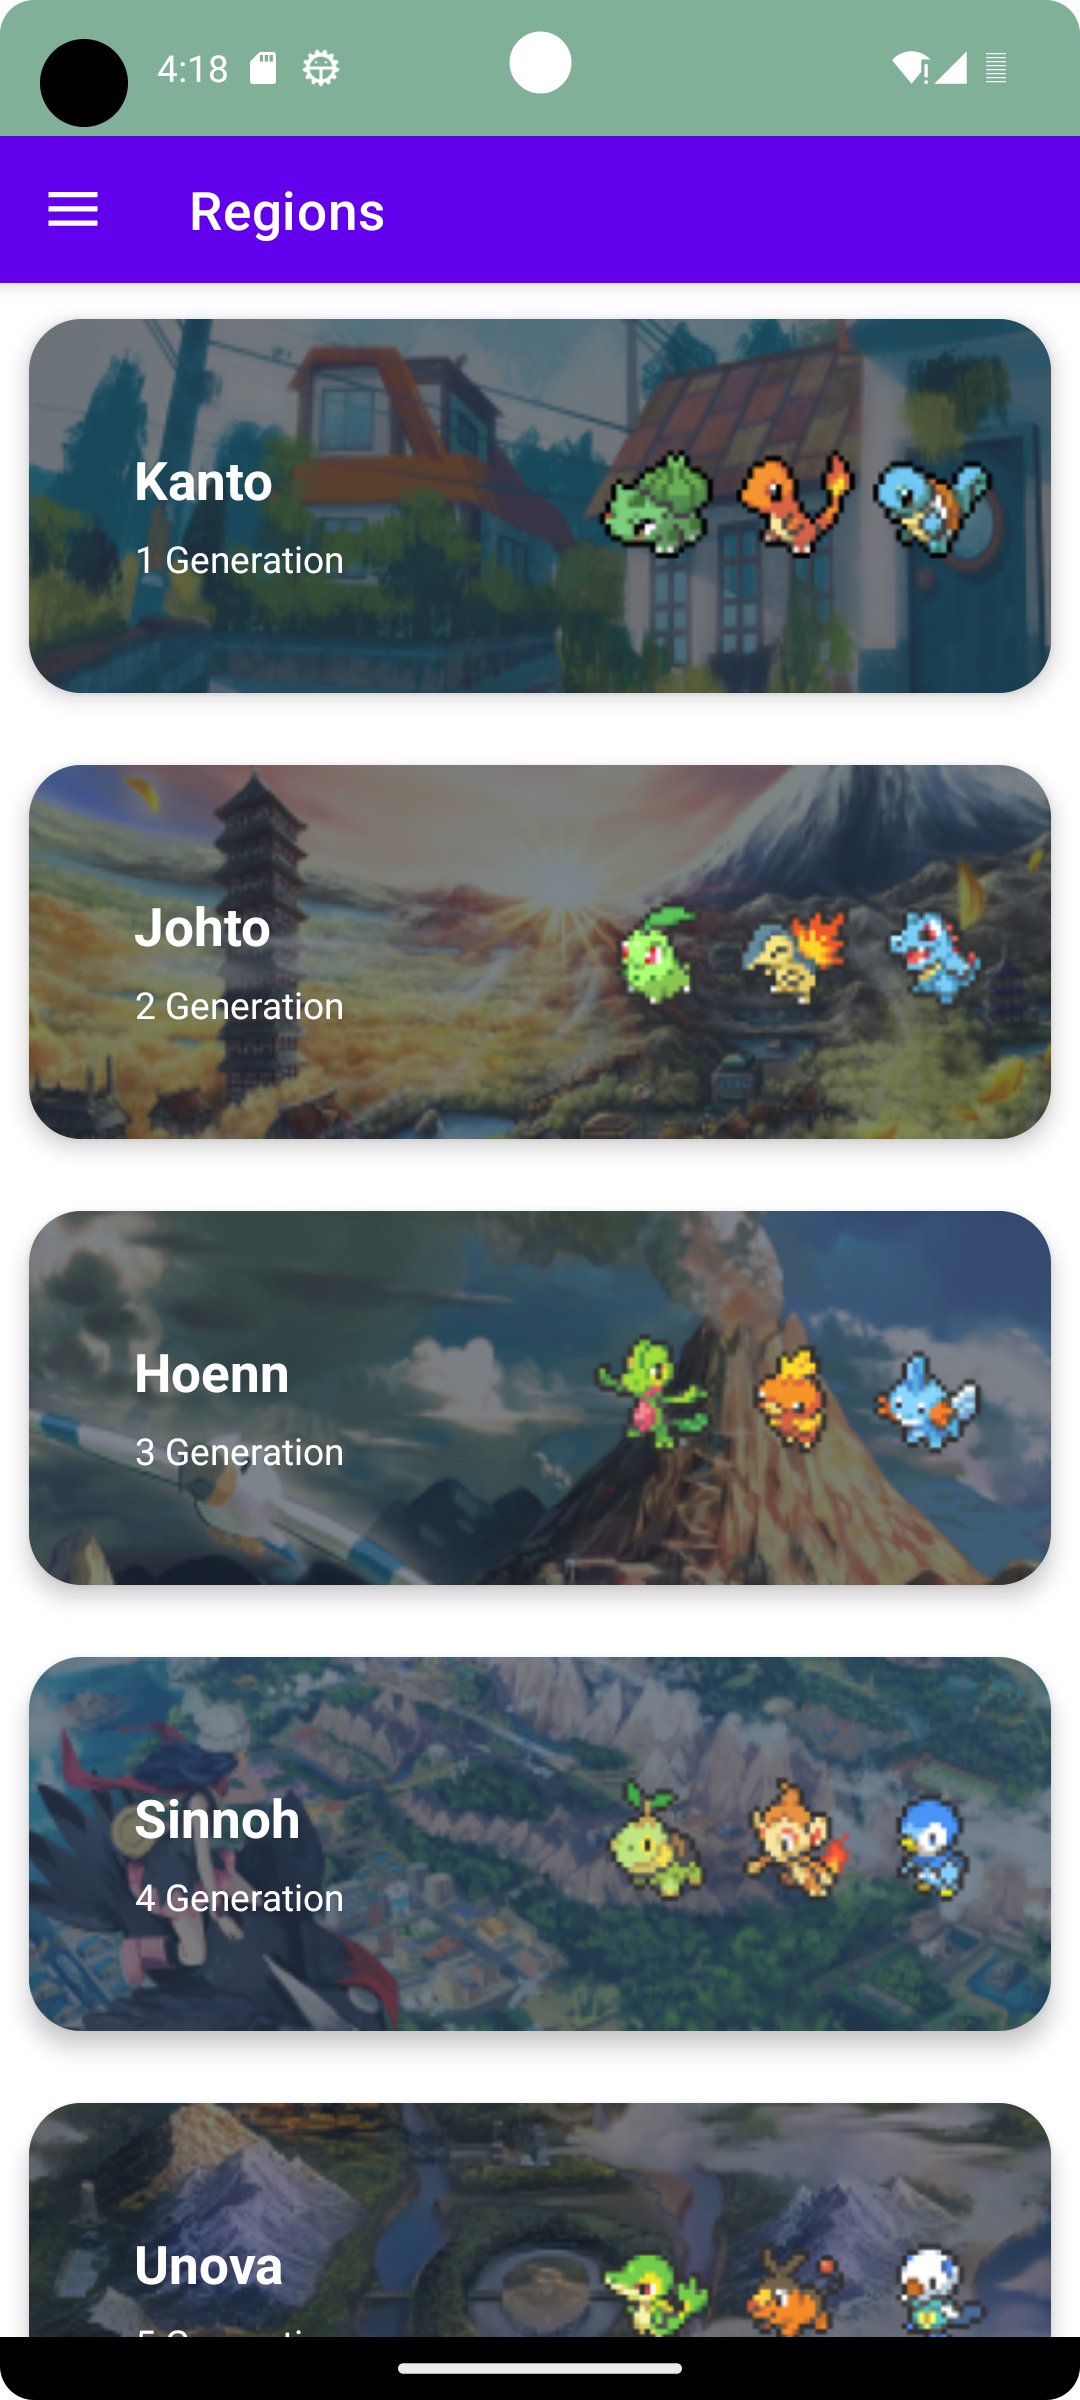
\includegraphics[height=7cm]{imgs/screens/screen_region.png}
	\caption{Screen List Pokemon Regions}
	\label{fig:screen_pokemon_regions}
\end{figure}


\begin{figure}[h]
	\centering
	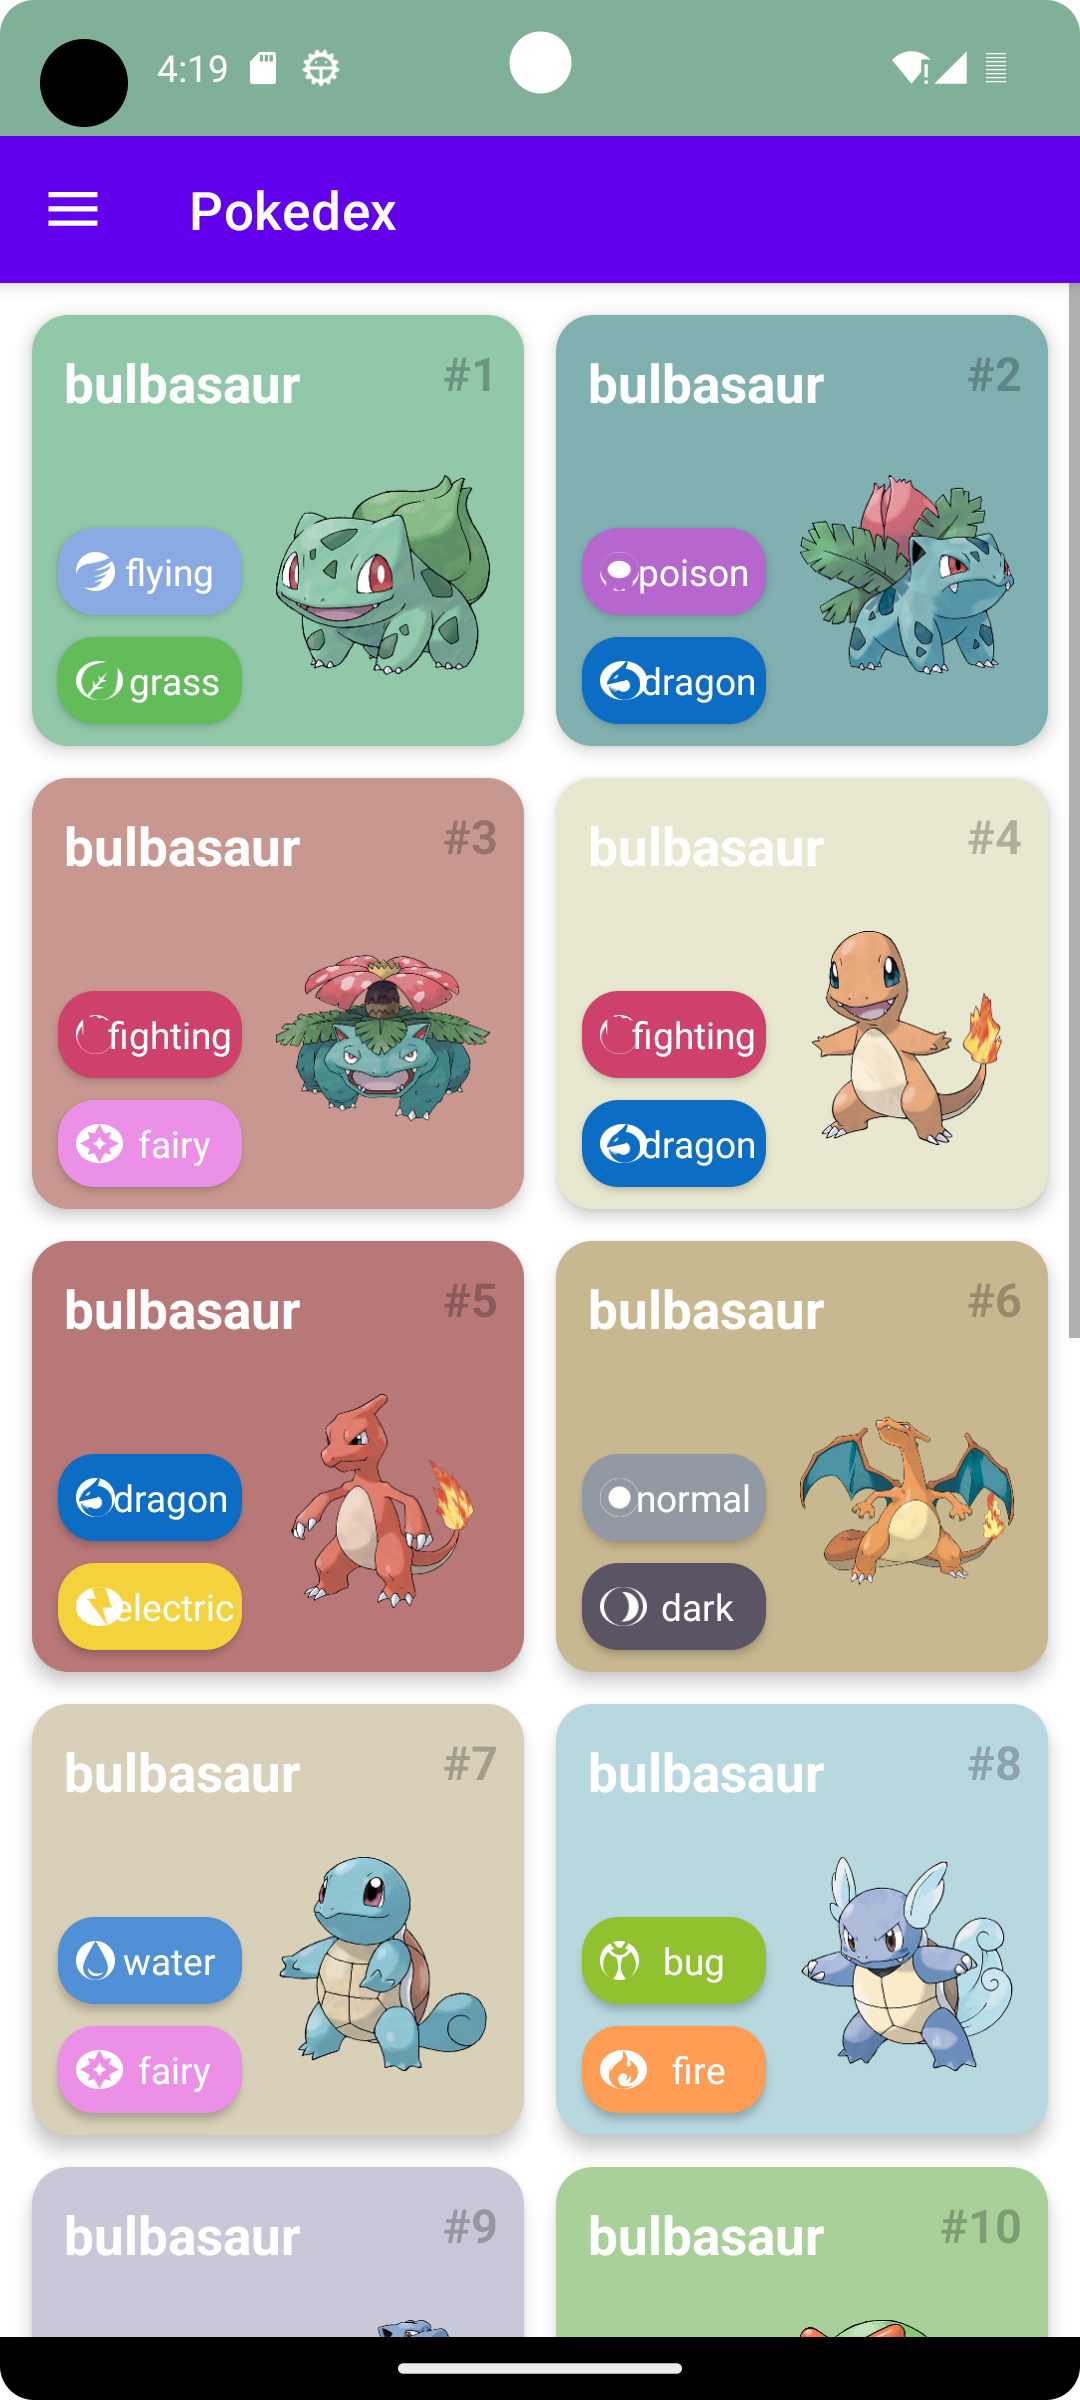
\includegraphics[height=7cm]{imgs/screens/screen_pokemons.png}
	\caption{Screen List Pokemons}
	\label{fig:screen_pokemons}
\end{figure}


\begin{figure}[h]
	\centering
	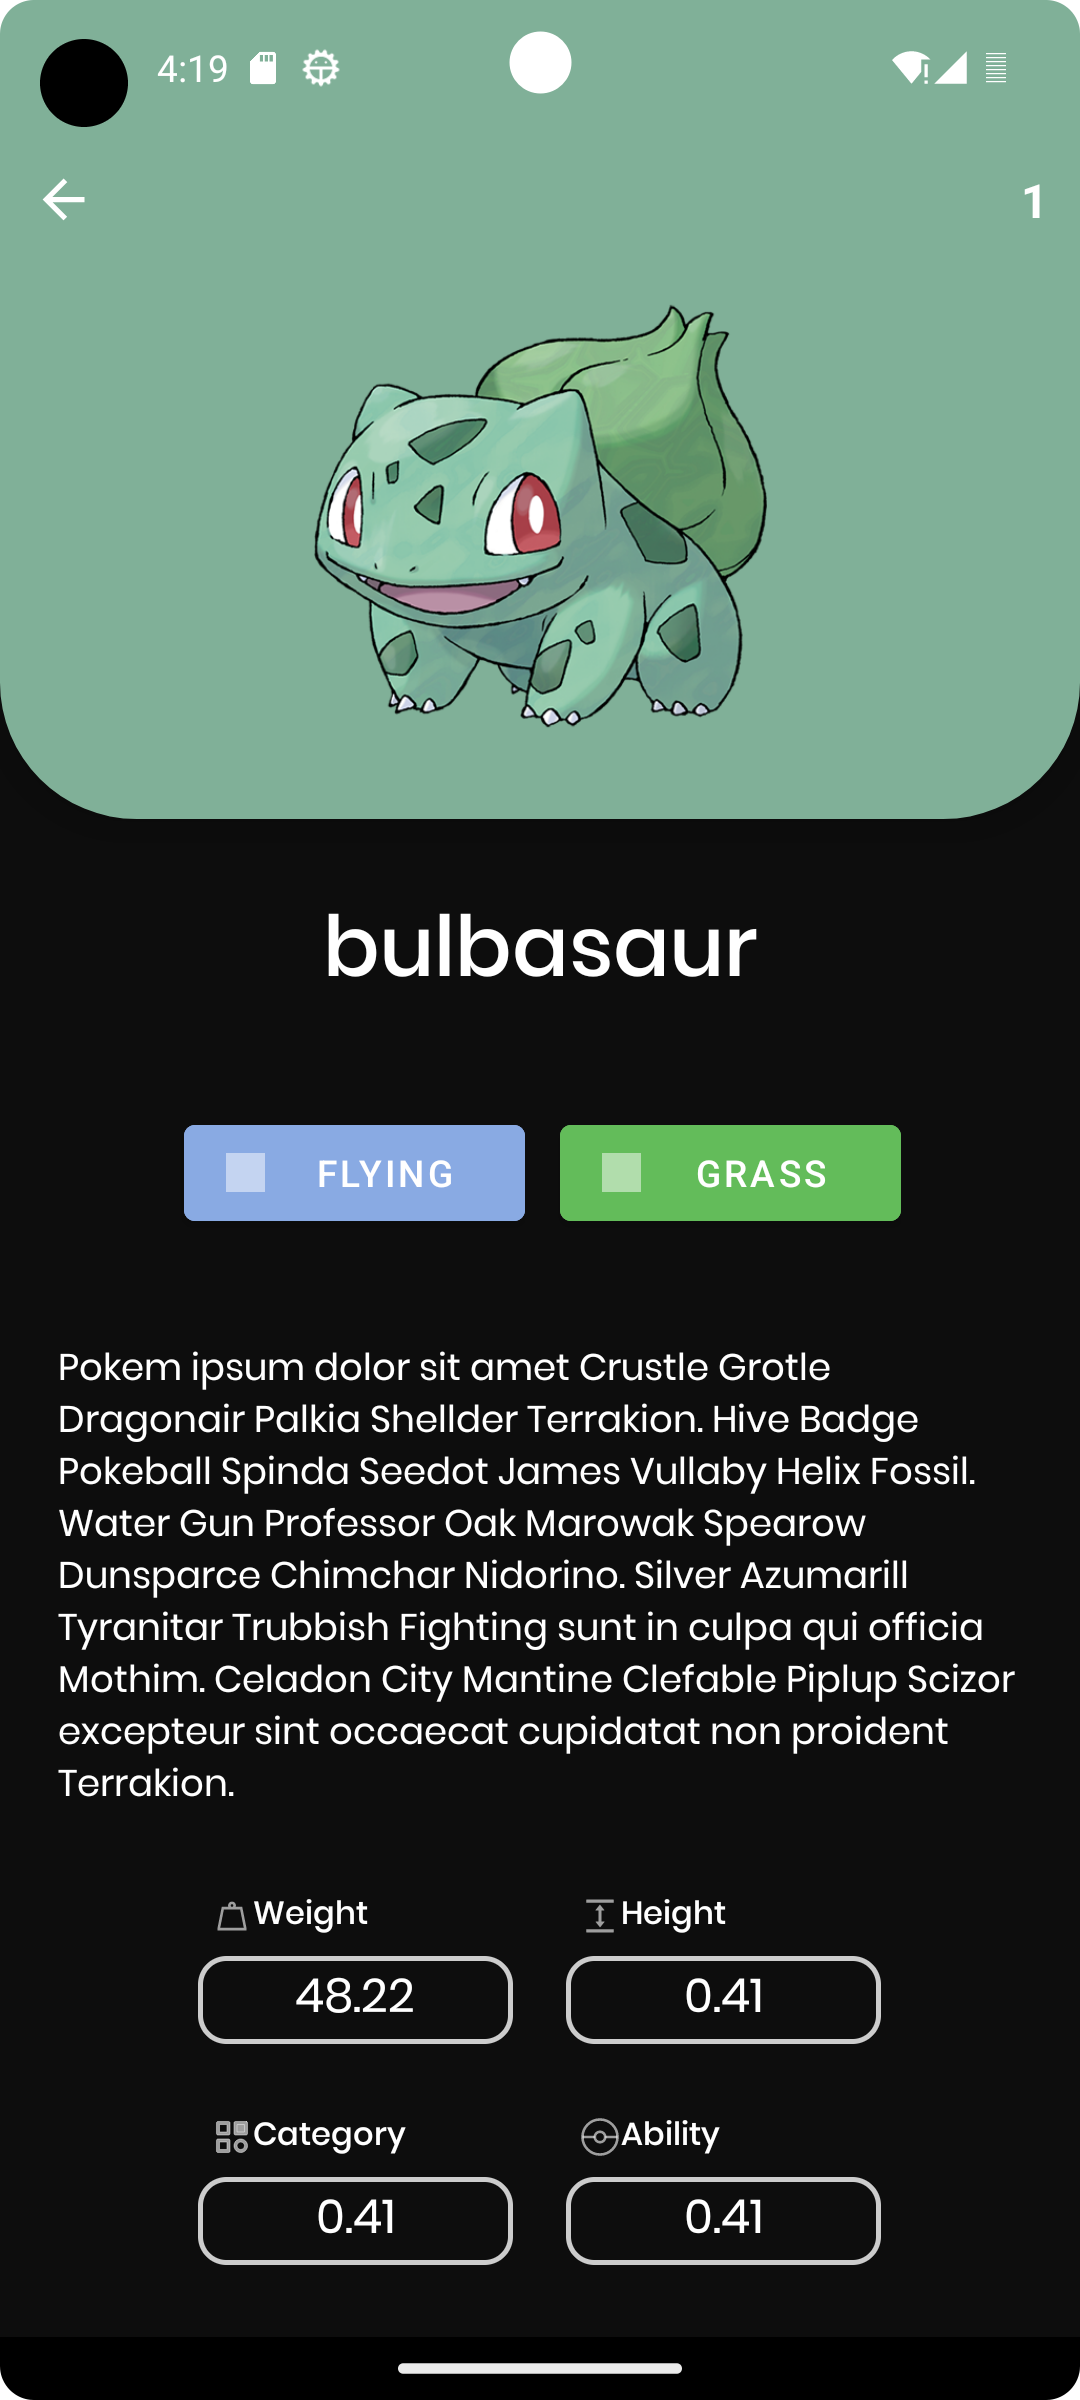
\includegraphics[height=7cm]{imgs/screens/screen_pokemon_detail.png}
	\caption{Screen Pokemon Detail}
	\label{fig:screen_pokemon_detail}
\end{figure}


%%%%%%%%%%%%%%%%%%%%%%%%%%%%%%%%%%%%%%%%%%%%%%%%%%%%%%%%%%%%%%%%%%

\section{Clean Architecture}

\textit{Clean Architecture} is a software architectural pattern for developing Android applications that focuses on separation of concerns, testability, and maintainability. 
It provides a structured approach to organizing code into different layers, each with a specific responsibility. 
These layers interact with each other in a specific way to create a modular and scalable architecture.

The main layers in Clean Architecture for Android are:

\begin{enumerate}
    \item \textbf{Presentation Layer}: This layer is responsible for rendering the user interface and handling user interactions. 
    It includes components such as activities, fragments, views, or view models (depending on the chosen architecture pattern, such as \textit{MVP} or \textit{MVVM}). 
    The presentation layer is responsible for displaying data to the user and capturing user inputs, but it should not contain business logic or data manipulation.
     It communicates with the domain layer to request data and trigger actions based on user interactions.

    \item \textbf{Domain Layer}: Also known as the business logic layer, this layer encapsulates the core logic of the application. 
    It includes use cases (or interactors) that represent the individual actions or operations that can be performed by the application. 
    Use cases are independent of any framework or external dependencies and define the business rules and logic of the application. 
    The domain layer communicates with the data layer to fetch or store data, and it defines the contracts or interfaces that are implemented by the data layer.
    
    \item \textbf{Data Layer}: This layer is responsible for fetching and storing data from external sources, such as databases, APIs, or repositories.
     It includes components such as data sources, repositories, and mappers that handle data conversion between different layers. 
     The data layer implements the contracts or interfaces defined in the domain layer and provides the data in a format suitable for the domain layer. 
     The data layer may also handle caching, offline data access, or other data-related operations.
    
\end{enumerate}

The iterations in Clean Architecture refer to the flow of data and control between the layers. 
The typical flow of data and control in Clean Architecture is as follows:

\begin{enumerate}
    \item The Presentation Layer communicates with the Domain Layer to request data or trigger actions based on user interactions.
    \item The Domain Layer contains the business logic and rules of the application and communicates with the Data Layer to fetch or store data.
    \item The Data Layer is responsible for fetching and storing data from external sources and implementing the contracts or interfaces defined in the Domain Layer.
    \item The Data Layer provides the requested data back to the Domain Layer, which then processes it and returns the result to the Presentation Layer.
    \item The Presentation Layer renders the user interface or takes appropriate actions based on the data received from the Domain Layer.
    
\end{enumerate}

It's important to note that Clean Architecture promotes a one-way flow of data and control, with dependencies pointing inward, from the outer layers to the inner layers. 
This ensures that the inner layers, such as the Domain Layer, are independent of any framework or external dependencies, making them highly testable and maintainable.

%%%%%%%%%%%%%%%%%%%%%%%%%%%%%%%%%%%%%%%%%%%%%%%%%%%%%%%%%%%%%%%%%%

\section{JetPack}

Most Android apps now use the support libraries to help users add all kinds of updated widgets and to address compatibility issues across Android devices and OS versions. You’d be hard-pressed to find an Android app that doesn’t use something from them, and they’re included as a dependency in template projects made in Android Studio. Widgets as fundamental as RecyclerView are included in them.

The support libraries are great to use, but they have evolved quite a bit over the years and the names have become somewhat confusing. 
There are com.android.support:support-v4 and com.android.support:support-v13, for example. Looking at the names alone, do you know what classes are in them? 
The names are supposed to designate what version of Android they support, but, as they have evolved, the minimum version has increased to API Level 14.

Google has realized that this variety of ever-changing libraries is very confusing for new (and old) developers and has decided to start over. 
Consequently, it has created Android Jetpack that is of components, tools and guidelines, that aims to facilitate the creation of applications.
As shown in Figure~\ref{fig:jetpackCategories}, the Android Jetpack components bring together
the support library which is a group of components that facilitate the use
of the new Android features and the Architecture Components that was
designed to facilitate data management during system changes
application lifecycle. The components are organized into four
categories:

\begin{enumerate}
	\item Architecture;
	\item UI;
	\item Behavior;
	\item Foundation.
\end{enumerate}


\begin{figure}[h]
	\centering
	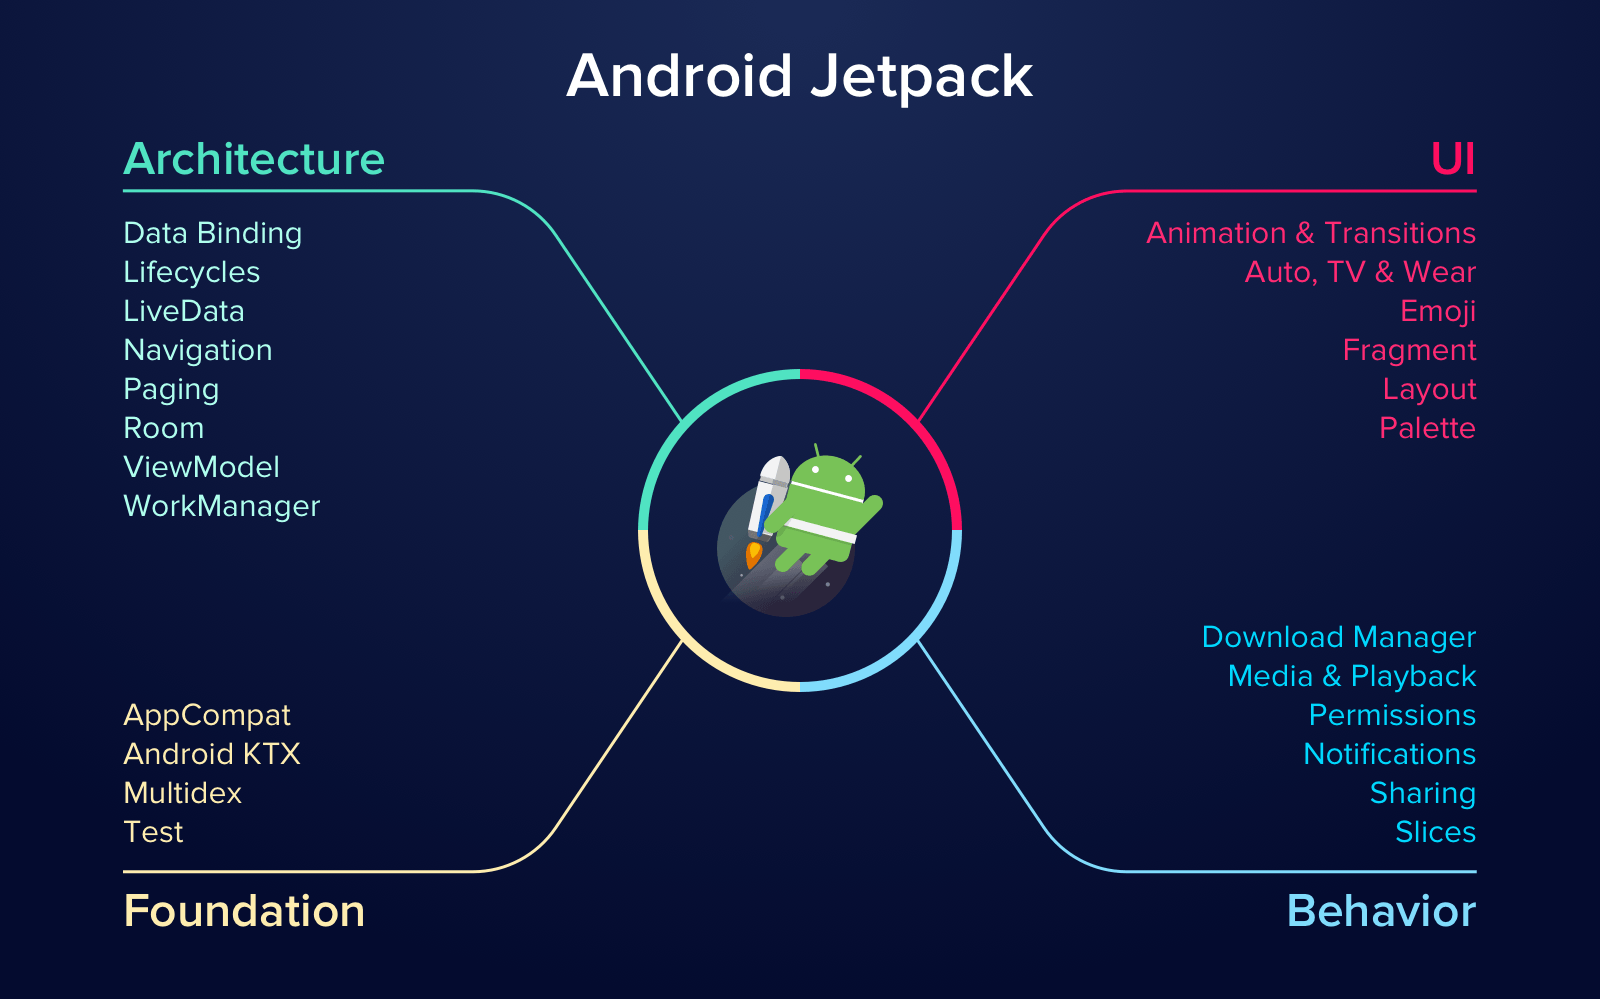
\includegraphics[height=10cm]{imgs/jetpack.png}
	\caption{Android Jetpack Categories.}
	\label{fig:jetpackCategories}
\end{figure}

\subsection{Architecture Components}

It is a collection of libraries that help to develop applications
robust, testable and easy to maintain. This library helps to manage the
life cycle of UI components and better control the persistence of
data even with changes in the application life cycle.
In the next topics we present the most importants libraries that make
part of Architecture Components.

\subsubsection{Room}
If you have ever struggled working with the SQLite database in an Android app, you will appreciate what the Room library does for you. You create several simple classes that define your data and how to access them, and the Room library will do most of the rest. The only SQL code you have to write is for queries, which are usually pretty straightforward. And you gain compile-time checks of your SQL code when using Room.

There are three important classes you need to use with Room: Database (this contains your main entry point and holds a reference to the database object for the app), Entity (you create one for each table in the database), and DAO (this contains the methods for retrieving and managing the data).

\subsubsection{Lifecycle}
The Lifecycle library helps you listen for lifecycle events in other components besides an activities and fragments. This allows you to have lifecycle-aware logic in places other than just an Activity or Fragment. The library works by using annotations on methods so you get notified for the events that you are interested in.

You implement LifecycleObserver, annotate methods and add this observer to a lifecycle owner, which is usually an Activity or Fragment. The LifecycleObserver class can get the current lifecycle state by calling lifecycle.getCurrentState() and can use this information to avoid calling code when not in the correct state.

A LifecycleOwner is an object that has Android lifecycle events. The support library Activity and Fragment classes already implement the LifecycleOwner methods. A LifecycleOwner has a Lifecycle object that it can return to let the observer know what the current state is.
\subsubsection{ViewModel}
While the Room library persists your data in permanent storage, the ViewModel class allows you to hold onto data in device memory in a lifecycle-aware manner. One of the nice features of a ViewModel is that it can survive the re-construction of an Activity or Fragment over a configuration change such as a device rotation. The system will hold onto that ViewModel re-associate it with the Activity or Fragment. ViewModels are also where you can load data in the background and use LiveData to notify listeners that the data is ready.

\subsubsection{LiveData}
The LiveData library uses the Observer pattern for data but handles it in a lifecycle-aware manner. You get the benefits of automatic UI updates when data changes without calling UI elements when the UI is not in the correct state.

LiveData is the class that implements the observer pattern, holds that data, and notifies listeners when that data has changed.
\subsubsection{Paging}
Have you ever had to deal with large amounts of related data? Maybe too much for you to download at once? The Paging library will help by providing ways to handle the paging of data in a RecyclerView.

The Paging library uses several key classes: PagedList, PagedListAdapter, and DataSource. PagedList is a list that loads data lazily from a DataSource, allowing the app to load data in chunks or pages. PagedListAdapter is a custom RecyclerView.Adapter that handles pages with a DiffUtil callback.

For the DataSource, you will use one of three different subclasses: PageKeyedDataSource, ItemKeyedDataSource, or PositionalDataSource.
\subsubsection{WorkManager}
Over the years, there have been several systems built into Android for handling background jobs or alarms. They differ on different versions of Android and you have to write a lot of code to handle the different versions of the OS.

WorkManager solves this problem and gives you one library for creating deferrable, asynchronous tasks and defining when they should run. You can define one-time jobs or repeating jobs.



%%%%%%%%%%%%%%%%%%%%%%%%%%%%%%%%%%%%%%%%%%%%%%%%%%%%%%%%%%%%%%%%%%

\section{MVVM in android}

MVVM (Model-View-ViewModel) is a widely used architectural pattern in Android app development that provides a clear separation of concerns and promotes a modular, maintainable, and testable codebase. 
When used in conjunction with Clean Architecture, MVVM can help create scalable and maintainable Android applications. 
Here's how MVVM can be implemented in Clean Architecture in an Android app using Jetpack components:

\begin{enumerate}
    \item Model: The Model in MVVM represents the data and business logic of the application. In Clean Architecture, it typically includes the following components:
    \item Entity: It represents the domain model, which is a pure Kotlin/Java representation of the data entities in the application. It contains only data and no business logic.
    \item Repository: It acts as an interface between the data sources (e.g., local database, remote server) and the domain layer. It defines the contract for accessing and managing data, and it can implement different data sources based on the application's requirements.
    \item Use Case/Interactor: It encapsulates the business logic of the application, defining the different use cases or interactions that can be performed by the application. It communicates with the repositories to fetch or modify data and defines the input and output models for each use case.
    \item View: The View represents the UI components of the application, including activities, fragments, and views. In MVVM, the View is passive and only responsible for displaying data and capturing user input. It does not contain any business logic. The View observes the ViewModel and updates the UI based on the data received from the ViewModel.
    \item ViewModel: The ViewModel acts as an intermediary between the View and the Model. It holds the UI-related state and business logic of the View. It exposes data to the View through observable properties, and it receives input from the View through commands or events. The ViewModel communicates with the Model to fetch or modify data and maps the data into a format that can be easily consumed by the View. The ViewModel is also responsible for handling UI-related events, such as user input validation and navigation.
    \item Data Binding: MVVM in Android often utilizes data binding, which is a feature provided by Android Jetpack. Data binding allows for declarative binding of UI components to data models, eliminating the need for manual UI updates. This means that the View automatically updates when the data in the ViewModel changes, and vice versa.
    \item Observables: Observables are used to enable communication between the View and the ViewModel. The ViewModel exposes observables (e.g., LiveData, ObservableField) that the View observes to get notified of data changes. When data changes in the Model or ViewModel, the observables emit notifications, which trigger updates in the View.
    \item Jetpack Components: Android Jetpack provides several components that can be used in MVVM, such as LiveData and ViewModel. 
    LiveData is a lifecycle-aware observable data holder that can be used to expose data from the ViewModel to the View, and it automatically handles UI updates based on the lifecycle of the View. 
    ViewModel is a lifecycle-aware component that is designed to store and manage UI-related data, and it survives configuration changes, such as screen rotations.
    
\end{enumerate}


%%%%%%%%%%%%%%%%%%%%%%%%%%%%%%%%%%%%%%%%%%%%%%%%%%%%%%%%%%%%%%%%%%


\section{Let's Start}

In this tutorial, the focus will be mainly on the Presentation layer, although for testability, the base model of the application will be implemented, and fictitious (mock) data and some rules will be used in the Domain layer. In Tutorial 4, the focus will be on the Model and Domain layers.

First, create a new project using the "Navigation Drawer Activity" template, which will create an application with a hamburger menu.

\begin{figure}
	\centering
	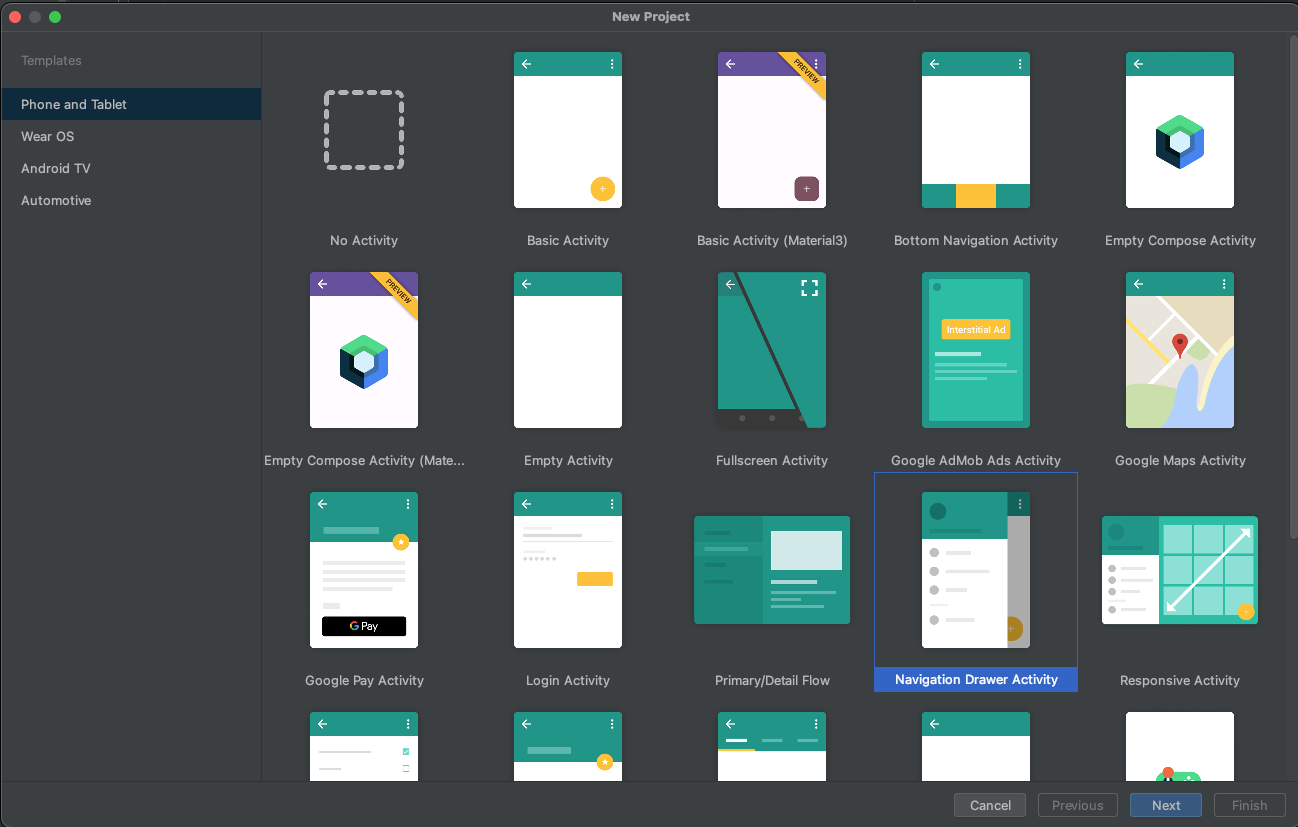
\includegraphics[height=10cm]{imgs/project/project_template.png}
	\caption{Project Template}
	\label{fig:pj_template}
\end{figure}

Before analyzing the project, you can delete some parts that will not be necessary for this tutorial:

\begin{enumerate}
    \item MainActivity: should only contain this code:

    \begin{lstlisting}[caption={Activity Main code.}, label={code:activity_main}, language=Kotlin]
        class MainActivity : AppCompatActivity() {

        private lateinit var appBarConfiguration: AppBarConfiguration
        private lateinit var binding: ActivityMainBinding
    
        override fun onCreate(savedInstanceState: Bundle?) {
            super.onCreate(savedInstanceState)
    
            binding = ActivityMainBinding.inflate(layoutInflater)
            setContentView(binding.root)
    
            setSupportActionBar(binding.appBarMain.toolbar)
    
            val drawerLayout: DrawerLayout = binding.drawerLayout
            val navView: NavigationView = binding.navView
            val navController = findNavController(R.id.nav_host_fragment_content_main)
            // Passing each menu ID as a set of Ids because each
            // menu should be considered as top level destinations.
            appBarConfiguration = AppBarConfiguration(
                setOf(
                    R.id.nav_regions, R.id.nav_gallery, R.id.nav_slideshow, R.id.nav_home
                ), drawerLayout
            )
            setupActionBarWithNavController(navController, appBarConfiguration)
             navView.setupWithNavController(navController)
        }
    
        override fun onSupportNavigateUp(): Boolean {
            val navController = findNavController(R.id.nav_host_fragment_content_main)
            return navController.navigateUp(appBarConfiguration) || super.onSupportNavigateUp()
        }
    }
    
\end{lstlisting}

    \item  Delete the \texttt{\detokenize{/menu/main.xml}} file.
    
    \item In the \texttt{\detokenize{layout/app_bar_main.xml}} file, only the following code should remain.
    

    \begin{lstlisting}[caption={App Bar Code.}, label={layout:app_bar_main_code}, language=XML]

    <androidx.coordinatorlayout.widget.CoordinatorLayout xmlns:android="http://schemas.android.com/apk/res/android"
        xmlns:app="http://schemas.android.com/apk/res-auto"
        xmlns:tools="http://schemas.android.com/tools"
        android:layout_width="match_parent"
        android:layout_height="match_parent"
        tools:context=".MainActivity">
    
        <com.google.android.material.appbar.AppBarLayout
            android:layout_width="match_parent"
            android:layout_height="wrap_content"
            android:theme="@style/Theme.DAMPokedexPart1.AppBarOverlay">
    
            <androidx.appcompat.widget.Toolbar
                android:id="@+id/toolbar"
                android:layout_width="match_parent"
                android:layout_height="?attr/actionBarSize"
                android:background="?attr/colorPrimary"
                app:popupTheme="@style/Theme.DAMPokedexPart1.PopupOverlay" />
    
        </com.google.android.material.appbar.AppBarLayout>
    
        <include layout="@layout/content_main" />
    </androidx.coordinatorlayout.widget.CoordinatorLayout>

\end{lstlisting}

\end{enumerate}

In the Moodle, you will find a zip file with the resources that will be used in the project.
These resources are divided into the following folders:

\begin{enumerate}
    \item drawable
    \item strings
    \item colors
\end{enumerate}
You should copy or import these files into the new project.

Add to /build.gradle the following lines in correct places:

\begin{lstlisting}[caption={/build.gradle.}, label={code:gradle}, language=XML]
    plugins {
        ...
        id 'org.jetbrains.kotlin.kapt'
        id 'kotlin-parcelize'
    }

    android { 
        ...
        buildFeatures {
            viewBinding true
            dataBinding true
        }
    }

    dependencies {

    ...

    /* Glide Libraries for download images using urls*/
    implementation 'com.github.bumptech.glide:glide:4.15.0'
    annotationProcessor 'com.github.bumptech.glide:compiler:4.15.0'

    /* Palette Library for obtain colors from images */
    implementation 'androidx.palette:palette:1.0.0'

    /* Progress View library */
    implementation "com.github.skydoves:progressview:1.1.3"
    }
    
\end{lstlisting}


Add to AndroidManifest the following lines:

\begin{lstlisting}[caption={Android Manifest}, label={code:android_manifest}, language=XML]
    <uses-permission android:name="android.permission.INTERNET" />
    <uses-permission android:name="android.permission.ACCESS_NETWORK_STATE" />
\end{lstlisting}


So let's start to implement the Pokedex APP 

And create the following packages(Figure~\ref{fig:pj_packges_clean_architecture}):

\begin{enumerate}
	\item ui - Contains all the classes of UI (Fragments and ViewModels).
	\item domain - Contains the classes that handle uses cases operations.
	\item data - Contains the application's data model classes.
\end{enumerate}

\begin{figure}[h]
	\centering
	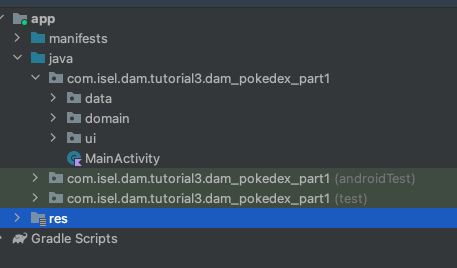
\includegraphics[height=7cm]{imgs/project/project_packges.png}
	\caption{Project packages}
	\label{fig:pj_packges_clean_architecture}
\end{figure}




\subsection{Basic Data Layer and Basic Domain}

We will create the necessary basic entities of our data model to be able to test the application.

\begin{enumerate}
    \item \textbf{PokemonRegion}:  which will contain the base information of the region - \textit{id, name, backgroundImage, startersImage} - \ref{code:pk_region_class}
    \item \textbf{Pokemon}: which will contain the base information of the pokemon - \textit{id, name, imageUrl, regions, types} - \ref{code:pk_class}
    \item \textbf{PokemonDetail}: which will contain the detailed information of the pokemon - \textit{id, pokemon, description, weight, height, stats, evolutions} - \ref{code:pk_detail_class}
    \item \textbf{PokemonType}: which will contain the information of the pokemon type - \textit{id, name, iconImage, color} - \ref{code:pk_type_class}
    \item \textbf{PokemonEvolution}: which will contain the information of the pokemon Evolution chain - \textit{id, pokemon} - \ref{code:pk_evolution_class}
    \item \textbf{PokemonStats}: which will contain the information of the pokemon "powers" - \textit{id, hp, attack, defense, specialDefence, speed, experience} - \ref{code:pk_stats_class}
\end{enumerate}

As one of the requirements of the application is to consume data using the POKEAPI, but we will only implement it in the next tutorial, it is necessary to use mock data to test the application. 
For this purpose, we will create the static object \textit{PokemonMockData}, which is located in the package \textit{data/mocks} \ref{code:mockData}.


We will also create the necessary basic functions to obtain data for testing the application.

\begin{lstlisting}[caption={Region Fragment Layout.}, label={code:screen_region_list}, language=Kotlin]
    class PokemonDomain
    {
        fun getAllRegions() : LiveData<List<PokemonRegion>>
        {
            return MutableLiveData<List<PokemonRegion>>(PokemonMockData.regions)
        }
        
        fun getAllPokemons(): LiveData<List<Pokemon>>
        {
            return MutableLiveData<List<Pokemon>>(PokemonMockData.pokemons)
        }
    
        fun getPokemonsByRegion(region: PokemonRegion): LiveData<List<Pokemon>>
        {
            return MutableLiveData<List<Pokemon>>(PokemonMockData.pokemons.filter { it.region == region })
        }
    
        fun getPokemonTypes(): List<PokemonType>
        {
            return ArrayList<PokemonType>(PokemonMockData.pokemonTypeMock)
        }
    
        fun getPokemonDetail(pokemon:Pokemon): LiveData<PokemonDetail>
        {
            return MutableLiveData(
                PokemonMockData.pokemonDetail.find { it.pokemon == pokemon })
        }
    }
    
\end{lstlisting}


\section{First Feature - Region List}

Create a fragment where shows the list of regions of the pokemon, like the Figure \ref{fig:screen_region}

\begin{figure}
	\centering
	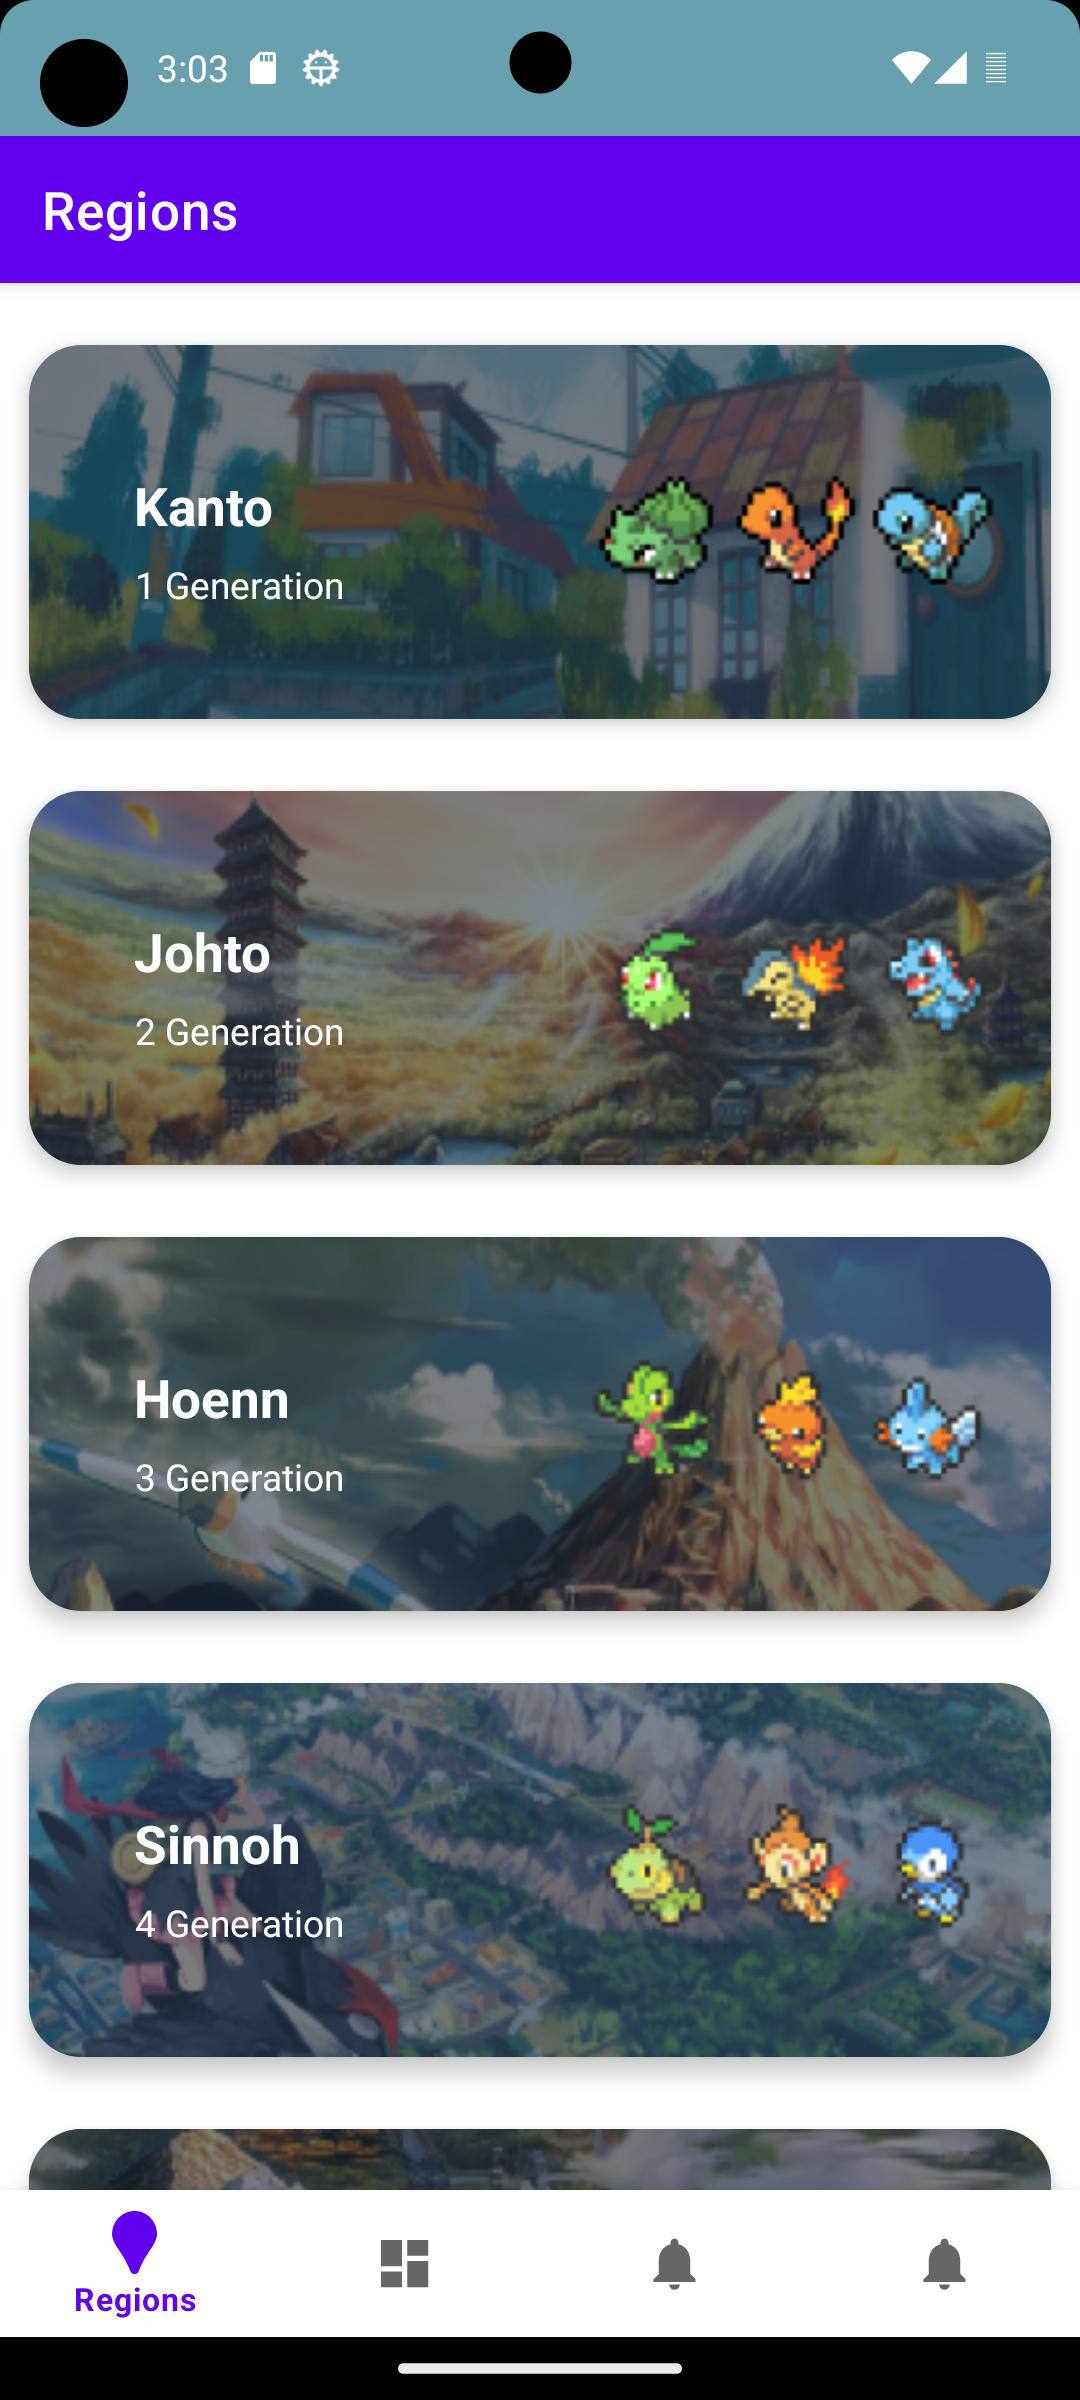
\includegraphics[height=10cm]{imgs/region_screen.png}
	\caption{Region Screen.}
	\label{fig:screen_region}
\end{figure}

\subsection{RecyclerView}

RecyclerView is an advanced and flexible version of ListView, which is a commonly used widget in Android to display a scrollable list of data. RecyclerView 
is part of the Android Jetpack library and offers several advantages over ListView, such as better performance, extensibility, 
and a more flexible layout manager system. RecyclerView recycles the views that are no longer visible on the screen, 
reducing the memory usage of the app and improving its performance.
The RecyclerView consists of three main components:
\begin{enumerate}
    \item \textbf{Layout Manager}: It is responsible for measuring and positioning the items in the RecyclerView. It can be either a built-in layout manager like LinearLayoutManager, GridLayoutManager, or StaggeredGridLayoutManager, or a custom layout manager.
    \item \textbf{Adapter}: It is responsible for providing the views that represent the data items in the RecyclerView. It creates a view holder for each item and binds the data to the views in the ViewHolder.
    \item \textbf{ViewHolder}: It holds the views that represent the data items in the RecyclerView. It provides a reference to these views so that the adapter can bind the data to them.
\end{enumerate}

First let's create the Fragment with View Model with the name \textit{RegionFragment} and in layout let's create a a RecyclerView with the LinearLayoutManager:

\begin{lstlisting}[caption={Region Fragment Layout.}, label={code:screen_region_list}, language=XML]
    <?xml version="1.0" encoding="utf-8"?>
    <FrameLayout xmlns:android="http://schemas.android.com/apk/res/android"
        xmlns:tools="http://schemas.android.com/tools"
        android:layout_width="match_parent"
        android:layout_height="match_parent"
        xmlns:app="http://schemas.android.com/apk/res-auto"
        tools:context=".ui.region.RegionFragment">
    
        <androidx.recyclerview.widget.RecyclerView
            android:id="@+id/regionsRecyclerView"
            android:layout_width="match_parent"
            android:layout_height="match_parent"
            app:layoutManager="LinearLayoutManager"/>
    
    </FrameLayout>
\end{lstlisting}

Second, let's create the region item layout, for that you have to add a new Layout Resource File and add the fowolling xml code:

\begin{lstlisting}[caption={Region Item Layout.}, label={code:screen_item_region}, language=XML]
    <?xml version="1.0" encoding="utf-8"?>
    <androidx.appcompat.widget.LinearLayoutCompat android:id="@+id/relativeLayoutBackground"
        android:layout_width="match_parent"
        android:layout_height="170dp"
        android:clickable="true"
        android:clipToPadding="true"
        android:focusable="true"
        xmlns:android="http://schemas.android.com/apk/res/android"
        xmlns:app="http://schemas.android.com/apk/res-auto"
        xmlns:tools="http://schemas.android.com/tools">
    
            <com.google.android.material.card.MaterialCardView
                android:layout_width="match_parent"
                android:layout_height="170dp"
                android:layout_margin="0dp"
                app:cardCornerRadius="20dp"
                app:cardElevation="5dp"
                app:cardPreventCornerOverlap="true"
                app:cardUseCompatPadding="true"
                android:padding="0dp">
    
                <androidx.appcompat.widget.AppCompatImageView
                    android:id="@+id/regionBgImage"
                    android:layout_width="match_parent"
                    android:layout_height="match_parent"
                    android:scaleType="fitXY"
                    android:foreground="#96222f3e"
                    android:foregroundTintMode="src_in"
                    tools:src="@drawable/bg_hoenn"/>
    
    
                <androidx.appcompat.widget.AppCompatImageView
                    android:id="@+id/regionStartersImageView"
                    android:layout_width="197dp"
                    android:layout_height="120dp"
                    android:layout_gravity="center|right"
                    android:layout_margin="0dp"
                    android:contentDescription="@string/app_name"
                    android:scaleType="center"
                    tools:src="@drawable/pk_hoenn"/>
    
                <androidx.appcompat.widget.AppCompatTextView
                    android:id="@+id/regionNameTextView"
                    android:layout_width="wrap_content"
                    android:layout_height="wrap_content"
                    android:layout_gravity="left|center_vertical"
                    android:layout_marginStart="40dp"
                    android:layout_marginBottom="10dp"
                    android:gravity="center|left"
                    android:textColor="@color/white"
                    android:textSize="20sp"
                    android:textStyle="bold"
                    tools:text="Hoenn"/>
    
                <androidx.appcompat.widget.AppCompatTextView
                    android:id="@+id/regionIdTextView"
                    android:layout_width="wrap_content"
                    android:layout_height="wrap_content"
                    android:layout_gravity="left|center_vertical"
                    android:layout_marginLeft="40dp"
                    android:layout_marginTop="20dp"
                    android:gravity="center"
                    android:textColor="@color/white"
                    android:textSize="14sp"
                    android:textStyle="bold"
                    app:fontFamily="sans-serif-thin"
                    tools:text="3 Generation"/>
            </com.google.android.material.card.MaterialCardView>
    
        </androidx.appcompat.widget.LinearLayoutCompat>
    
\end{lstlisting}

Third, let's create the \textit{Region Adapter} with the ViewHolder.


\begin{lstlisting}[caption={Region Adapter Class.}, label={code:screen_region_adapter}, language=Kotlin]
    class RegionAdapter(
    private val pkRegionList: List<PokemonRegion>,
    private val context: Context
) : RecyclerView.Adapter<RegionAdapter.ViewHolder>() {

    class ViewHolder(itemView: View) : RecyclerView.ViewHolder(itemView) {
        private val viewBinding = ItemRegionBinding.bind(itemView)
        fun bindView(regionItem: PokemonRegion)
        {
            viewBinding.regionNameTextView.text = regionItem.name
            viewBinding.regionIdTextView.text = "${regionItem.id} ${R.string.pk_generations}".uppercase()
            viewBinding.regionBgImage.setImageDrawable(ContextCompat.getDrawable(itemView.context,regionItem.bg))
            viewBinding.regionStartersImageView.setImageDrawable(ContextCompat.getDrawable(itemView.context,regionItem.starters))
            itemView.setOnClickListener{
                Toast.makeText(itemView.context, String.format("Click in %s Region", regionItem.name), Toast.LENGTH_LONG).show()
            };
        }
    }

    override fun onCreateViewHolder(parent: ViewGroup, viewType: Int): ViewHolder {
        val inflater = LayoutInflater.from(context)
        val view = inflater.inflate(R.layout.item_region, parent, false)
        return ViewHolder(view)
    }

    override fun onBindViewHolder(holder: ViewHolder, position: Int) {
        val item = pkRegionList[position]
        holder.bindView(item)
    }

    override fun getItemCount(): Int {
        return pkRegionList.size
    }

}
\end{lstlisting}

The Adapter is a crucial component of the RecyclerView as it provides a bridge between the data source and the views that represent that data in the RecyclerView. The Adapter is responsible for creating and managing the ViewHolder objects, which are responsible for holding references to the views that represent each item in the RecyclerView. The Adapter also binds the data to the views in the ViewHolder.

The Adapter class is an abstract class, and you need to extend it and implement its three methods:

\begin{enumerate}
    \item \textbf{onCreateViewHolder()} : This method creates a new ViewHolder object for each item in the RecyclerView. It inflates the layout for the item view and returns a new instance of the ViewHolder.
    \item \textbf{onBindViewHolder()}: This method binds the data to the views in the ViewHolder. It takes the position of the item in the data source and updates the views in the ViewHolder with the corresponding data.
    \item \textbf{getItemCount()}: This method returns the total number of items in the data source.

\end{enumerate}

In the constructor of the RegionAdapter class, the list of PokemonRegion objects and a context are passed as parameters. The context is used to create a LayoutInflater instance, which is used to inflate the item layout.

The ViewHolder class is defined as a nested class within the adapter, and it extends the RecyclerView.ViewHolder class. In the ViewHolder class, the view binding is done using the ItemRegionBinding class, which is generated by the Android Data Binding Library. The bindView() method is used to bind the view with the data for a single item in the list.

In the onCreateViewHolder() method, the item layout is inflated and a ViewHolder instance is created and returned.

In the onBindViewHolder() method, the data for a single item is retrieved from the list, and the ViewHolder's bindView() method is called to bind the view with the data.

Finally, the getItemCount() method is used to return the number of items in the list.

Third create the \textit{RegionViewModel} aims to obtain the list of regions that are exist in pokemon franchise.

\begin{lstlisting}[caption={Region View Model Class.}, label={code:code_region_vm}, language=Kotlin]
    class RegionViewModel : ViewModel()
    {
        private val _pokemonDomain = PokemonDomain()
    
        fun getRegions(): LiveData<List<PokemonRegion>>
        {
            return _pokemonDomain.getAllRegions()
        }
    }

\end{lstlisting}

ViewModels offer a number of benefits:

\begin{enumerate}
	\item ViewModel‘s are lifecycle-aware, which means they know when the attached Activity/Fragment is destroyed and can immediately release data observers and other resources.
	\item They survive configuration changes, so if your data is observed or fetched through a ViewModel, it’s still available after your Activity or Fragment is re-created. This means you can re-use the data without fetching it again.
	\item ViewModel takes the responsibility of holding and managing data. It acts as a bridge between your Repository and the View. Freeing up your Activity or Fragment from managing data allows you to write more concise and unit-testable code.
\end{enumerate}

To enable the usage of view models in your Android application, add the following snippet to the app/build.gradle file.

\begin{lstlisting}[caption={Region Fragment.}, label={code:gradle_vm}, language=XML]
	android {
		....
		buildFeatures {
			viewBinding true
		}
	}
\end{lstlisting}

For the last, lets connect all this components in Fragment:

\begin{lstlisting}[caption={View Models Gradle.}, label={code:fragment_region}, language=Kotlin]
	class RegionFragment : Fragment() {

    private var _regionViewModel: RegionViewModel?  = null

    private var _binding: FragmentRegionBinding? = null

    private val binding get() = _binding!!

    private val regionViewModel get() = _regionViewModel!!

    override fun onCreateView(
        inflater: LayoutInflater,
        container: ViewGroup?,
        savedInstanceState: Bundle?
    ): View {
        _regionViewModel =
            ViewModelProvider(this)[RegionViewModel::class.java]

        _binding = FragmentRegionBinding.inflate(inflater, container, false)

        return binding.root
    }

    override fun onViewCreated(view: View, savedInstanceState: Bundle?) {
        super.onViewCreated(view, savedInstanceState)

        regionViewModel.getRegions().observe(viewLifecycleOwner) {
            val regions: List<PokemonRegion> = it
            binding?.regionsRecyclerView?.adapter = RegionAdapter(regions, view.context)
        }
    }

    override fun onDestroyView() {
        super.onDestroyView()
        _binding = null
    }
}
\end{lstlisting}

In the \textit{onCreateView()} method, the fragment inflates its layout using the FragmentRegionBinding class.
 This class is generated by the Android Data Binding Library and provides a type-safe way to access views in the layout. 
 The \textit{RegionViewModel} is also initialized using the ViewModelProvider class.

In the \textit{onViewCreated()} method, the RecyclerView adapter is set up using the RegionAdapter class, which takes a list of PokemonRegion objects and a context.
The adapter is set on the RecyclerView using the binding object, which is the instance of 
FragmentRegionBinding that was created in the \textit{onCreateView()} method. The adapter is updated whenever the data in the RegionViewModel changes.

So lets testing this feature, for that we have to do little changes in app navigation.

Jetpack Navigation is a library provided by Google to simplify the navigation process between different screens (Fragments, Activities) in an Android application. With Jetpack Navigation, developers can easily create a navigation graph that maps out the different screens in their app and the possible paths between them.

The Jetpack Navigation library provides several benefits for developers:

\begin{enumerate}
    \item Simplified Navigation: Jetpack Navigation provides a simple and consistent way to navigate between different screens in an Android application. It eliminates the need for developers to write boilerplate code to handle navigation, which can be tedious and error-prone.

    \item Type-safe navigation: Jetpack Navigation uses the Safe Args plugin to generate type-safe classes for passing arguments between different screens. This ensures that developers can catch errors early in the development process and avoid runtime crashes due to passing the wrong data type between screens.
    
    \item Back Stack Management: Jetpack Navigation provides automatic back stack management for fragments. This means that when the user presses the back button, the application automatically navigates back to the previous screen, instead of exiting the app.
 
\end{enumerate}


Open the file \textit{mobilenavigation.xml} in the folder \textit{res/navigation}.

\begin{lstlisting}[caption={Navigation Code.}, label={code:nav_code}, language=XML]
	<navigation xmlns:android="http://schemas.android.com/apk/res/android"
    xmlns:app="http://schemas.android.com/apk/res-auto"
    xmlns:tools="http://schemas.android.com/tools"
    android:id="@+id/mobile_navigation"
    app:startDestination="@+id/nav_home">

    <fragment
        android:id="@+id/nav_home"
        android:name="com.isel.dam.tutorial3.dam_pokedex_part1.ui.home.HomeFragment"
        android:label="@string/menu_home"
        tools:layout="@layout/fragment_home" >

    </fragment>

    <fragment
        android:id="@+id/nav_gallery"
        android:name="com.isel.dam.tutorial3.dam_pokedex_part1.ui.gallery.GalleryFragment"
        android:label="@string/menu_gallery"
        tools:layout="@layout/fragment_gallery" />

    <fragment
        android:id="@+id/nav_slideshow"
        android:name="com.isel.dam.tutorial3.dam_pokedex_part1.ui.slideshow.SlideshowFragment"
        android:label="@string/menu_slideshow"
        tools:layout="@layout/fragment_slideshow" />
   
</navigation>
\end{lstlisting}

This is an XML code that defines the navigation graph for an Android application using Jetpack Navigation.
A navigation graph is a collection of destinations, which represent different screens in the app, and the actions that connect them.

The navigation graph is defined using the \textit{<navigation>} tag with the following attributes:

\textbf{android:id} sets the ID for the navigation graph to \texttt{\detokenize{mobile_navigation}}.
\textbf{app:startDestination} sets the starting destination to \texttt{\detokenize{nav_home}}.
The navigation graph contains four fragments, each represented by the \textbf{<fragment>} tag:

\begin{enumerate}
    \item \textbf{\texttt{\detokenize{nav_home}}} is the home screen of the app and is defined by the HomeFragment class.
    \item \textbf{\texttt{\detokenize{nav_gallery}}} is a gallery screen and is defined by the GalleryFragment class.
    \item \textbf{\texttt{\detokenize{nav_slideshow}}} is a slideshow screen and is defined by the SlideshowFragment class.
\end{enumerate}

Each <fragment> tag specifies the following attributes:

\begin{enumerate}
    \item \textbf{android:id} sets the ID for the fragment.
    \item \textbf{android:name} sets the fully qualified name of the fragment's class.
    \item \textbf{android:label} sets the label that is displayed for the fragment in the app's navigation drawer or toolbar.
    \item \textbf{tools:layout} specifies the layout resource for the fragment's view.
\end{enumerate}

The navigation graph represents the hierarchy of the app's screens and the transitions between them. It enables the app to manage and handle user navigation in a structured and organized manner.

Let's add the Region Fragment to our navigation graph:

\begin{lstlisting}[caption={Navigation with Region Fragment.}, label={code:nav_region_code}, language=XML]
	<navigation xmlns:android="http://schemas.android.com/apk/res/android"
    xmlns:app="http://schemas.android.com/apk/res-auto"
    xmlns:tools="http://schemas.android.com/tools"
    android:id="@+id/mobile_navigation"
    app:startDestination="@+id/nav_home">

    <fragment
        android:id="@+id/nav_home"
        android:name="com.isel.dam.tutorial3.dam_pokedex_part1.ui.home.HomeFragment"
        android:label="@string/menu_home"
        tools:layout="@layout/fragment_home" >

    </fragment>

    <fragment
        android:id="@+id/nav_gallery"
        android:name="com.isel.dam.tutorial3.dam_pokedex_part1.ui.gallery.GalleryFragment"
        android:label="@string/menu_gallery"
        tools:layout="@layout/fragment_gallery" />

    <fragment
        android:id="@+id/nav_slideshow"
        android:name="com.isel.dam.tutorial3.dam_pokedex_part1.ui.slideshow.SlideshowFragment"
        android:label="@string/menu_slideshow"
        tools:layout="@layout/fragment_slideshow" />

    <fragment
        android:id="@+id/nav_regions"
        android:name="com.isel.dam.tutorial3.dam_pokedex_part1.ui.region.RegionFragment"
        android:label="@string/menu_regions"
        tools:layout="@layout/fragment_region" />
   
</navigation>
\end{lstlisting}

And add the Regions option to Drawer Menu in \textit{\texttt{\detokenize{res/menu/activity_main_drawer}}}:

\begin{lstlisting}[caption={Navigation with Region Fragment.}, label={code:nav_region_code}, language=XML]
    <item
    android:id="@+id/nav_regions"
    android:icon="@drawable/ic_region"
    android:title="@string/menu_regions" />
\end{lstlisting}

\subsection{Data Binding}

Data Binding is a feature provided by Android Jetpack that allows you to bind UI components in your layout directly to data sources in your app's code.
 This means you can avoid writing a lot of boilerplate code to update your UI components with data from your app.

To use Data Binding in this app, you need to enable it by adding the following to your module's build.gradle file:


\begin{lstlisting}[caption={Navigation with Region Fragment.}, label={code:nav_region_code}, language=XML]
    android {
		....
		buildFeatures {
			databinding true
		}
	}
\end{lstlisting}

Once you've enabled Data Binding, you can start using it in your layout files by enclosing
your layout in a <layout> tag. 
Within the <layout> tag, you can use the @{} syntax to bind data to UI components. 
For example in Region item Layout, you can bind a string to a \textit{regionIdTextView} and \textit{regionNameTextView} like this:


\begin{lstlisting}[caption={Navigation with Region Fragment.}, label={code:nav_region_code}, language=Kotlin]
    <layout xmlns:android="http://schemas.android.com/apk/res/android"
    xmlns:app="http://schemas.android.com/apk/res-auto"
    xmlns:tools="http://schemas.android.com/tools">

    <data>
        <variable
            name="region"
            type="com.isel.dam.tutorial3.dam_pokedex.data.model.PokemonRegion" />

    </data>
<androidx.appcompat.widget.LinearLayoutCompat
    android:id="@+id/relativeLayoutBackground"
    android:layout_width="match_parent"
    android:layout_height="170dp"
    android:clickable="true"
    android:clipToPadding="true"
    android:focusable="true">

    <com.google.android.material.card.MaterialCardView
        android:layout_width="match_parent"
        android:layout_height="170dp"
        android:layout_margin="0dp"
        app:cardCornerRadius="20dp"
        app:cardElevation="5dp"
        app:cardPreventCornerOverlap="true"
        app:cardUseCompatPadding="true"
        android:padding="0dp"

        >

        <androidx.appcompat.widget.AppCompatImageView
            android:layout_width="match_parent"
            android:id="@+id/regionBgImage"
            android:layout_height="match_parent"
            android:scaleType="fitXY"
            android:src="@{region.bg}"
            android:foreground="#96222f3e"
            android:foregroundTintMode="src_in"/>


        <androidx.appcompat.widget.AppCompatImageView
            android:id="@+id/regionStartersImageView"
            android:layout_width="197dp"
            android:layout_height="120dp"
            android:layout_gravity="center|right"
            android:layout_margin="0dp"
            android:contentDescription="@string/app_name"
            android:scaleType="center"
            android:src="@{region.starters}" />

        <androidx.appcompat.widget.AppCompatTextView
            android:id="@+id/regionTitleTextView"
            android:layout_width="wrap_content"
            android:layout_height="wrap_content"
            android:layout_gravity="left|center_vertical"
            android:layout_marginStart="40dp"
            android:layout_marginBottom="10dp"
            android:gravity="center|left"
            android:text="@{region.name}"
            android:textColor="@color/white"
            android:textSize="20sp"
            android:textStyle="bold" />

        <androidx.appcompat.widget.AppCompatTextView
            android:id="@+id/regionSubtitleTextView"
            android:layout_width="wrap_content"
            android:layout_height="wrap_content"
            android:layout_gravity="left|center_vertical"
            android:layout_marginLeft="40dp"
            android:layout_marginTop="20dp"
            android:gravity="center"
            android:text="@{Integer.toString(region.id)}"
            android:textColor="@color/white"
            android:textSize="14sp"
            android:textStyle="bold"
            app:fontFamily="sans-serif-thin" />



    </com.google.android.material.card.MaterialCardView>


</androidx.appcompat.widget.LinearLayoutCompat>
    </layout>
\end{lstlisting}

For the  \textit{regionBgImage} and \textit{regionStartersImageView} we need to create a custom binding for setting the image resource (src) of an ImageView, because we need translate integer to Bitmap 

\begin{lstlisting}[caption={Navigation with Region Fragment.}, label={code:nav_region_code}, language=Kotlin]
    object ViewBinding {

    @JvmStatic
    @BindingAdapter("android:src")
    fun setImageResource(imageView: AppCompatImageView, resource: Int) {
        imageView.setImageDrawable(ContextCompat.getDrawable(imageView.context,resource))
    }

}
\end{lstlisting}

\begin{enumerate}
    \item \textit{@JvmStatic}: This annotation is used to indicate that the function should be treated as a static method in Java. 
    This allows the function to be called from Java code as a static method, rather than as an instance method.
    \item \textit{@BindingAdapter("android:src")}: This is a custom binding adapter annotation provided by the Data Binding library.
    It specifies that this binding adapter is intended to be used to bind the "android:src" attribute of an ImageView in a layout XML file.
    \item \textit{fun setImageResource(imageView: AppCompatImageView, resource: Int)}: This is the definition of the binding adapter function. It takes two parameters:
    \begin{enumerate}
        \item \textit{imageView}: An instance of AppCompatImageView, which is the ImageView to which the binding adapter is being applied.
        \item \textit{resource}: An integer value, which represents the image resource ID that needs to be set as the source of the ImageView.
    \end{enumerate}
    imageView.setImageDrawable(ContextCompat.getDrawable(imageView.context, resource)): This line of code sets the image resource for the ImageView. 
        It uses the ContextCompat.getDrawable() method to retrieve a Drawable object from the given resource ID using the context of the ImageView,
         and then sets it as the drawable source of the ImageView using the setImageDrawable() method.
\end{enumerate}


We need to change the Adapter View Holder in \textit{bindView} to bind the property region:

\begin{lstlisting}[caption={Binding property Region.}, label={code:binding_region_code}, language=Kotlin]
    fun bindView(regionItem: PokemonRegion)
        {
            /*viewBinding.regionNameTextView.text = regionItem.name
            viewBinding.regionIdTextView.text = "${regionItem.id} ${R.string.pk_generations}".uppercase()
            viewBinding.regionBgImage.setImageDrawable(ContextCompat.getDrawable(itemView.context,regionItem.bg))
            viewBinding.regionStartersImageView.setImageDrawable(ContextCompat.getDrawable(itemView.context,regionItem.starters))*/
            viewBinding.region = regionItem
            itemView.setOnClickListener{
                Toast.makeText(itemView.context, String.format("Click in %s Region", regionItem.name), Toast.LENGTH_LONG).show()
            };
        }
}
\end{lstlisting}

Let's test the Region Fragment:

Go to \textit{\texttt{\detokenize{res/navigation/mobile_navigation.xml}}} and add the RegionFragments using the icon screen with green plus and change the id Fragment to "\textit{\texttt{\detokenize{nav_regions}}}"
Go to \textit{\texttt{\detokenize{res/menu/activity_main_drawer.xml}}} and new item:

\begin{lstlisting}[caption={Add new Menu item.}, label={xml:menu_new_item}, language=XML]
    <item
    android:id="@+id/nav_regions"
    android:icon="@drawable/ic_region"
    android:title="@string/menu_regions" />
\end{lstlisting}

Go to \textit{\texttt{\detokenize{MainActivity}}} and change the AppBarConfiguration:

\begin{lstlisting}[caption={Add new Menu item.}, label={xml:menu_new_item}, language=Kotlin]
    appBarConfiguration = AppBarConfiguration(
        setOf(
            R.id.nav_regions, R.id.nav_gallery, R.id.nav_slideshow, R.id.nav_home
        ), drawerLayout
    )
    
\end{lstlisting}

\section{Pokemon List}

Create a new layout \textit{\texttt{\detokenize{item_pokemon.xml}}}

\begin{lstlisting}[caption={Binding property Region.}, label={code:binding_region_code}, language=XML]
    <?xml version="1.0" encoding="utf-8"?>
<layout xmlns:android="http://schemas.android.com/apk/res/android"
    xmlns:app="http://schemas.android.com/apk/res-auto"
    xmlns:tools="http://schemas.android.com/tools">

    <data>

        <variable
            name="pokemon"
            type="com.isel.dam.tutorial3.dam_pokedex_part1.data.model.Pokemon" />

    </data>

    <com.google.android.material.card.MaterialCardView
        android:id="@+id/cardView"
        android:layout_width="match_parent"
        android:layout_height="wrap_content"
        android:layout_margin="6dp"
        android:foreground="?attr/selectableItemBackground"
        app:cardBackgroundColor="@color/white"
        app:cardCornerRadius="14dp"
        app:cardElevation="4dp"
        app:layout_constraintEnd_toEndOf="parent"
        app:layout_constraintStart_toStartOf="parent"
        app:layout_constraintTop_toTopOf="parent"
        tools:cardBackgroundColor="@color/water">

        <androidx.constraintlayout.widget.ConstraintLayout
            android:layout_width="match_parent"
            android:layout_height="wrap_content"
            android:foreground="?attr/selectableItemBackground"
            app:cardBackgroundColor="@color/white">

            <androidx.appcompat.widget.AppCompatImageView
                android:id="@+id/image"
                android:layout_width="90dp"
                android:layout_height="90dp"
                android:layout_margin="20dp"
                android:layout_marginStart="10dp"
                android:layout_marginTop="5dp"
                android:layout_marginEnd="10dp"
                android:layout_marginBottom="10dp"
                android:adjustViewBounds="true"
                android:scaleType="fitCenter"
                app:layout_constraintBottom_toBottomOf="parent"
                app:layout_constraintEnd_toEndOf="parent"
                app:layout_constraintStart_toEndOf="@+id/pokemonType1"
                app:layout_constraintTop_toBottomOf="@+id/pokemonID"
                app:paletteCard="@{cardView}"
                app:paletteImage="@{pokemon.imageUrl}"

                tools:src="@drawable/charmander"/>

            <androidx.appcompat.widget.AppCompatTextView
                android:id="@+id/name"
                android:layout_width="wrap_content"
                android:layout_height="wrap_content"
                android:elevation="4dp"
                android:gravity="center"
                android:maxLines="1"
                android:padding="12dp"
                android:text="@{pokemon.name}"
                android:textColor="@color/white"
                android:textSize="20sp"
                android:textStyle="bold"
                app:layout_constraintStart_toStartOf="parent"
                app:layout_constraintTop_toTopOf="parent"
                tools:text="Charmander"/>

            <androidx.appcompat.widget.AppCompatTextView
                android:id="@+id/pokemonID"
                android:layout_width="wrap_content"
                android:layout_height="wrap_content"
                android:layout_marginTop="10dp"
                android:layout_marginEnd="10dp"
                android:alpha="0.25"
                android:gravity="top"
                android:textColor="@color/black"
                android:textSize="18sp"
                android:textStyle="bold"
                android:text="@{@string/pk_id(pokemon.id)}"
                app:layout_constraintEnd_toEndOf="parent"
                app:layout_constraintTop_toTopOf="parent"
                tools:text="#4"/>


            <androidx.cardview.widget.CardView
                android:id="@+id/pokemonType1"
                android:layout_width="70dp"
                android:layout_height="wrap_content"
                android:layout_marginStart="10dp"
                android:layout_marginBottom="50dp"
                android:maxWidth="20dp"
                app:cardBackgroundColorType="@{pokemon.types[0].color}"
                app:cardCornerRadius="14dp"
                app:cardElevation="2dp"
                app:layout_constraintBottom_toBottomOf="parent"
                app:layout_constraintStart_toStartOf="parent"
                tools:cardBackgroundColor="@color/fire">


                <androidx.constraintlayout.widget.ConstraintLayout
                    android:layout_width="match_parent"
                    android:layout_height="match_parent"
                    android:padding="2dp">

                    <androidx.appcompat.widget.AppCompatImageView
                        android:id="@+id/imageView4"
                        android:layout_width="15dp"
                        android:layout_height="15dp"
                        android:layout_marginStart="5dp"
                        android:layout_marginTop="5dp"
                        android:layout_marginBottom="5dp"
                        android:background="@drawable/bg_image_pokemon_type"
                        android:scaleType="fitCenter"
                        android:src="@{pokemon.types[0].icon}"
                        app:layout_constraintBottom_toBottomOf="parent"
                        app:layout_constraintStart_toStartOf="parent"
                        app:layout_constraintTop_toTopOf="parent"
                        app:srcCompat="@drawable/bug"
                        tools:src="@drawable/fire"/>

                    <androidx.appcompat.widget.AppCompatTextView
                        android:id="@+id/textView3"
                        android:layout_width="wrap_content"
                        android:layout_height="wrap_content"
                        android:layout_marginStart="5dp"
                        android:layout_marginTop="5dp"
                        android:layout_marginEnd="10dp"
                        android:layout_marginBottom="5dp"
                        android:gravity="center|center_vertical"
                        android:text="@{pokemon.types[0].name}"
                        android:textColor="@color/white"
                        android:textSize="14sp"
                        app:layout_constraintBottom_toBottomOf="parent"
                        app:layout_constraintEnd_toEndOf="parent"
                        app:layout_constraintStart_toEndOf="@+id/imageView4"
                        app:layout_constraintTop_toTopOf="parent"
                        tools:text="Fire"/>
                </androidx.constraintlayout.widget.ConstraintLayout>
            </androidx.cardview.widget.CardView>


            <androidx.cardview.widget.CardView
                android:id="@+id/pokemonType2"
                android:layout_width="70dp"
                android:layout_height="wrap_content"
                android:layout_marginStart="10dp"
                android:layout_marginTop="20dp"
                android:layout_marginBottom="20dp"
                android:maxWidth="20dp"
                app:cardBackgroundColorType="@{pokemon.types[1].color}"
                app:cardCornerRadius="14dp"
                app:cardElevation="2dp"
                app:layout_constraintBottom_toBottomOf="parent"
                app:layout_constraintStart_toStartOf="parent"
                app:layout_constraintTop_toBottomOf="@+id/pokemonType1"
                tools:cardBackgroundColor="@color/bug">


                <androidx.constraintlayout.widget.ConstraintLayout
                    android:layout_width="match_parent"
                    android:layout_height="match_parent"
                    android:padding="2dp">

                    <androidx.appcompat.widget.AppCompatImageView
                        android:id="@+id/pokemonType2Icon"
                        android:layout_width="18dp"
                        android:layout_height="15dp"
                        android:layout_marginStart="5dp"
                        android:layout_marginTop="5dp"

                        android:layout_marginBottom="5dp"
                        android:background="@drawable/bg_image_pokemon_type"
                        android:scaleType="fitCenter"
                        android:src="@{pokemon.types[1].icon}"
                        app:layout_constraintBottom_toBottomOf="parent"
                        app:layout_constraintStart_toStartOf="parent"
                        app:layout_constraintTop_toTopOf="parent"
                        tools:src="@drawable/bug"/>

                    <androidx.appcompat.widget.AppCompatTextView
                        android:id="@+id/pokemonType2Label"
                        android:layout_width="wrap_content"
                        android:layout_height="wrap_content"
                        android:layout_marginStart="5dp"
                        android:layout_marginTop="5dp"
                        android:layout_marginEnd="10dp"
                        android:layout_marginBottom="5dp"
                        android:gravity="center|center_vertical"
                        android:text="@{pokemon.types[1].name}"
                        android:textColor="@color/white"
                        android:textSize="14sp"
                        app:layout_constraintBottom_toBottomOf="parent"
                        app:layout_constraintEnd_toEndOf="parent"
                        app:layout_constraintStart_toEndOf="@+id/pokemonType2Icon"
                        app:layout_constraintTop_toTopOf="parent"
                        tools:text="Bug"/>
                </androidx.constraintlayout.widget.ConstraintLayout>
            </androidx.cardview.widget.CardView>


        </androidx.constraintlayout.widget.ConstraintLayout>

    </com.google.android.material.card.MaterialCardView>

</layout>
}
\end{lstlisting}


\begin{lstlisting}[caption={New Custom Bindings.}, label={code:binding_region_code}, language=Kotlin]
    /**/
    @JvmStatic
    @BindingAdapter("app:cardBackgroundColorType")
    fun setCardBackgroundColor(carview: CardView, resource: Int)
    {
        carview.setCardBackgroundColor(ContextCompat.getColor(carview.context,resource))
    }

    /**/
    @JvmStatic
    @BindingAdapter("paletteImage", "paletteCard")
    fun bindLoadImagePalette(view: AppCompatImageView, url: String, paletteCard: MaterialCardView) {
        Glide.with(view.context)
            .asBitmap()
            .load(url)
            .listener(object : RequestListener<Bitmap>
            {
                override fun onLoadFailed(
                    e: GlideException?,
                    model: Any?,
                    target: com.bumptech.glide.request.target.Target<Bitmap>?,
                    isFirstResource: Boolean
                ): Boolean {

                    Log.d("TAG", e?.message.toString())
                    return false
                }

                override fun onResourceReady(
                    resource: Bitmap?,
                    p1: Any?,
                    p2: com.bumptech.glide.request.target.Target<Bitmap>?,
                    p3: DataSource?,
                    p4: Boolean
                ): Boolean {
                    Log.d("TAG", "OnResourceReady")
                    if (resource != null) {
                        val p: Palette = Palette.from(resource).generate()

                        val rgb = p?.lightMutedSwatch?.rgb
                        if (rgb != null) {
                            paletteCard.setCardBackgroundColor(rgb)


                        }
                    }
                    return false
                }
            })
            .into(view)
    }
\end{lstlisting}

The function \textit{bindLoadImagePalette} is responsible for binding an image loaded with Glide to an AppCompatImageView, and dynamically setting the background color of a MaterialCardView based on the palette of the loaded image.

The function has three parameters:
\begin{enumerate}
    \item view: An instance of AppCompatImageView, which represents the image view where the image will be loaded.
    \item url: A String parameter representing the URL of the image to be loaded.
    \item paletteCard: An instance of MaterialCardView, which represents the card view whose background color will be set based on the palette of the loaded image.
\end{enumerate}

Inside the function, Glide is used to load the image from the given URL (url) as a bitmap. The listener method is used to attach a custom implementation of 
RequestListener to handle events related to the image loading process.

The onLoadFailed method of the RequestListener is called if the image fails to load, and it logs the error message to the console.

The onResourceReady method of the RequestListener is called when the image is successfully loaded. Inside this method, the Palette library is used to generate a palette from the loaded image, and the lightMutedSwatch is used to get the RGB value of the dominant color in the light muted swatch. This RGB value is then used to set the background color of the MaterialCardView (paletteCard) using the setCardBackgroundColor method.

Finally, the into method is called to load the image into the AppCompatImageView (view) using Glide. The function returns false to indicate that the event is not consumed and should continue propagating to other listeners.

The function \textit{setCardBackgroundColor} is responsible for setting the background color of a CardView based on a resource ID, which represents a color value.

The function has two parameters:

\begin{enumerate}
    \item cardview: An instance of CardView, which represents the card view whose background color will be set.
    \item resource: An Int parameter representing the resource ID of the color value to be used as the background color of the CardView.
\end{enumerate}

Inside the function, the ContextCompat.getColor method is used to retrieve the color value associated with the given resource ID from the context of the CardView (carview.context).
This color value is then passed to the setCardBackgroundColor method of the CardView (carview) to set the background color accordingly.



\subsection{Pokemons Fragment and ViewModel}

Create a new Fragment \textit{PokemonsFragment} with ViewModel and go to \textit{\texttt{\detokenize{fragment_pokemons.xml}}} and create a RecyclerView.

\begin{lstlisting}[caption={Pokemons Fragment Layout.}, label={code:xml_pokemons_fragment}, language=XML]
<?xml version="1.0" encoding="utf-8"?>
<FrameLayout xmlns:android="http://schemas.android.com/apk/res/android"
    xmlns:tools="http://schemas.android.com/tools"
    android:layout_width="match_parent"
    android:layout_height="match_parent"
    xmlns:app="http://schemas.android.com/apk/res-auto"
    tools:context=".ui.pokemon.PokemonsFragment">

    <androidx.recyclerview.widget.RecyclerView
        android:id="@+id/pokemonsRecyclerView"
        android:layout_width="match_parent"
        android:layout_height="match_parent"
        android:layout_marginTop="0dp"
        android:layout_marginBottom="0dp"
        android:clipToPadding="false"
        android:fadeScrollbars="false"
        android:padding="6dp"
        android:scrollbarStyle="outsideOverlay"
        android:scrollbars="vertical"
        app:layoutManager="GridLayoutManager"
        app:spanCount="2"
        tools:listitem="@layout/item_pokemon"
        tools:spanCount="2"
        />

</FrameLayout>
\end{lstlisting}


\begin{lstlisting}[caption={Pokemons Fragment code.}, label={code:code_pokemons_fragment}, language=Kotlin]
    class PokemonsFragment : Fragment() {
        private var _binding: FragmentPokemonsBinding? = null
        private val viewModel: PokemonsViewModel by viewModels()
    
        private val binding get() = _binding!!
    
        override fun onCreateView(
            inflater: LayoutInflater,
            container: ViewGroup?,
            savedInstanceState: Bundle?
        ): View {
            _binding = FragmentPokemonsBinding.inflate(inflater, container, false)
            val root: View = binding.root
            return root
        }
    
        override fun onViewCreated(view: View, savedInstanceState: Bundle?) {
            super.onViewCreated(view, savedInstanceState)
    
            val region = checkNotNull(arguments?.getParcelable("region", PokemonRegion::class.java))
            viewModel.getListPokemonsByRegion(region).observe(viewLifecycleOwner, Observer {
                val pokemons: List<Pokemon> = it
                binding?.pokemonsRecyclerView?.adapter = PokemonsAdapter(pokemons,view.context)
            })
        }
    
        override fun onDestroyView() {
            super.onDestroyView()
            _binding = null
        }
    
    }
\end{lstlisting}

\begin{lstlisting}[caption={Pokemons ViewModel code.}, label={code:code_pokemons_vm}, language=Kotlin]
    class PokemonsViewModel : ViewModel() {

    private val pokemonDomain = PokemonDomain()

    private lateinit var listPokemons : LiveData<List<Pokemon>>

    fun getListPokemonsByRegion(region: PokemonRegion): LiveData<List<Pokemon>>
    {
        listPokemons = pokemonDomain.getPokemonsByRegion(region)
        return listPokemons
    }
}
\end{lstlisting}


\begin{lstlisting}[caption={Pokemons Adapter code.}, label={code:code_pokemons_adapter}, language=Kotlin]
    class PokemonsAdapter(
        private val pokemonList: List<Pokemon>,
        private val context: Context
    ) : RecyclerView.Adapter<PokemonsAdapter.ViewHolder>() {
    
        class ViewHolder(itemView: View) : RecyclerView.ViewHolder(itemView) {
            private val viewBinding = ItemPokemonBinding.bind(itemView)
            fun bindView(item: Pokemon) {
                viewBinding.pokemon = item
            }
        }
    
        override fun onCreateViewHolder(parent: ViewGroup, viewType: Int): ViewHolder {
    
            val inflater = LayoutInflater.from(context)
            val view = inflater.inflate(R.layout.item_pokemon, parent, false)
    
    
            return ViewHolder(view)
        }
    
        override fun onBindViewHolder(holder: ViewHolder, position: Int) {
            val item = pokemonList[position]
            holder.bindView(item)
        }
    
        override fun getItemCount(): Int {
            return pokemonList.size
        }
    
        companion object {
            private val POKEMON_DIFF_CALLBACK = object : DiffUtil.ItemCallback<Pokemon>() {
                override fun areItemsTheSame(oldItem: Pokemon, newItem: Pokemon): Boolean =
                    oldItem.id == newItem.id
    
                override fun areContentsTheSame(oldItem: Pokemon, newItem: Pokemon): Boolean =
                    oldItem == newItem
            }
        }
    
    }
\end{lstlisting}


With the Pokemon List feature already created, the desired behavior is to navigate to the Pokemon page and show only the Pokemon that belong to the selected region when clicking on a region.

To implement this use case, it is necessary to add the navigation behavior between these two fragments. 
For this, we will use the Jetpack Navigation Library, which is already included in the templates of this project.

\subsection{Navigation Android}

Jetpack Navigation is a set of libraries provided by Google as part of the Android Jetpack architecture components.
It aims to simplify the implementation of navigation and UI flow in Android apps by providing a declarative and graphical way to define navigation paths between different screens or destinations within an app.

At the core of Jetpack Navigation is the Navigation Graph, which is an XML resource that defines the structure of the app's navigation flow. 
The Navigation Graph contains a collection of destinations, which represent the individual screens or fragments in the app, and the actions or connections between these destinations.

The key components of Jetpack Navigation are:

\begin{enumerate}
    \item Navigation Graph: It is an XML resource that represents the navigation structure of the app. It defines the destinations (screens or fragments) in the app and the connections between them. 
    Destinations are defined with unique IDs and can have arguments, which are used to pass data between destinations. \textit{\texttt{\detokenize{res/navigation/mobile_navigation.xml}}} 

    \item NavHost: It is a container that hosts the fragments or screens defined in the Navigation Graph.
     It acts as a placeholder for the different destinations in the app and manages the navigation between them. 
     The NavHost is typically defined in the app's XML layout file and can be either a FragmentContainerView or a NavHostFragment.
     \textit{\texttt{\detokenize{res/layouts/contain_main.xml}}} 
    
    \item NavController: It is an object that manages the navigation between destinations in the app.
     It is responsible for handling user interactions, such as button clicks or gestures, 
     and navigating to the appropriate destinations based on the actions defined in the Navigation Graph.
    The NavController can be obtained using the Navigation.findNavController() method, passing in the NavHost as a parameter.

    \item Navigation Actions: These are connections between destinations in the Navigation Graph that define the possible navigation paths in the app. 
    Actions can be associated with user interactions, such as clicking a button, or triggered programmatically in code. 
    Actions can also have arguments, which are used to pass data between destinations.
    
    \item Navigation UI Components: Jetpack Navigation also provides UI components, such as NavigationView, BottomNavigationView, and Toolbar, that can be used to implement common navigation patterns, 
    such as a navigation drawer, bottom navigation bar, or an app bar with back and up buttons.
    \textit{\texttt{\detokenize{res/layouts/activity_main.xml}}} 
    
    \item Safe Args: It is a code generation plugin provided by Jetpack Navigation that generates type-safe arguments classes for passing data between destinations.
     It eliminates the need for manually handling argument bundles or parsing data from Intent extras, making the code safer and less error-prone.
    
\end{enumerate}

So, we need to modify the adapter so that when creating the cell for the region, when clicking on the cell, it navigates to the PokemonList page and passes the associated region object as an argument.

To avoid passing the NavController as an argument in the Adapter's constructor, a universal clickListener was created.
Create a new package \textit{ui/events} e add new kotlin File with following code:

\begin{lstlisting}[caption={Universal Click Listener.}, label={code:code_universal_listener_click}, language=Kotlin]

    typealias OnItemClickedListener = (arg: Any) -> Unit

\end{lstlisting}

In Kotlin, typealias is used to provide an alternative name for a function type or a complex type. 
It allows you to create a new name that can be used interchangeably with the original type.
In this case, the typealias OnItemClickedListener is defined as a function type that takes an argument of type Any and returns Unit. 
The Any type is a generic type that can represent any type of object, while Unit is a special type in Kotlin that indicates a function that doesn't return any value, similar to void in Java.
This typealias can be used to define a callback function that is invoked when an item is clicked in a UI component, such as a RecyclerView item or a button. 
The OnItemClickedListener can be used as a type for a function parameter or a property, making the code more concise and readable. 
When this callback is invoked, it will receive an argument of type Any, which can be cast or processed as needed within the function body.

In the  \textit{\texttt{\detokenize{res/navigation/mobile_navigation}}} , we will add the Pokemons Fragment and Regions Fragment and add the navigation action between RegionsFragment and PokemonsFragment by simply dragging the mouse from the RegionsFragment white point to the PokemonFragment.

\begin{figure}[h]
	\centering
	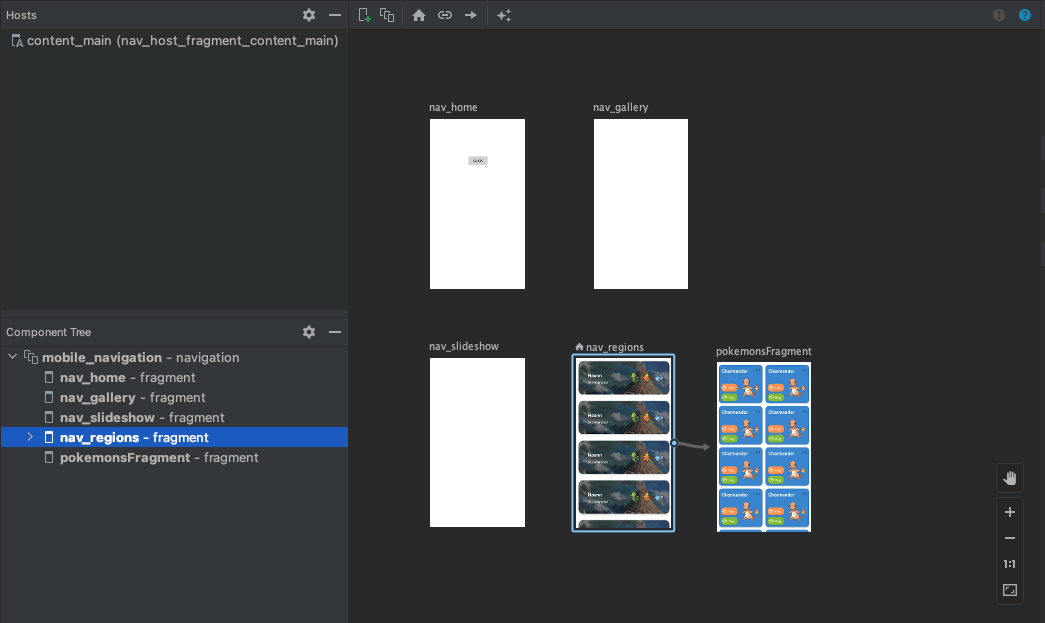
\includegraphics[height=7cm]{imgs/nav_xml.png}
	\caption{Navigation XML}
	\label{fig:pj_packges}
\end{figure}

\subsection{Modify Region Fragment and Adapter to navigato to Pokemons List}

\begin{lstlisting}[caption={Region Adapter to suport navigation code.}, label={code:code_region_adapter_nav}, language=Kotlin]
    class RegionAdapter(
    private val pkRegionList: List<PokemonRegion>,
    private val itemClickedListener: OnItemClickedListener? = null,
    private val context: Context
) : RecyclerView.Adapter<RegionAdapter.ViewHolder>() {

    class ViewHolder(itemView: View) : RecyclerView.ViewHolder(itemView) {
        private val viewBinding = ItemRegionBinding.bind(itemView)
        fun bindView(regionItem: PokemonRegion, itemClickedListener: OnItemClickedListener?)
        {
            /*viewBinding.regionNameTextView.text = regionItem.name
 viewBinding.regionIdTextView.text = String.format(itemView.context.getString(R.string.pk_generations), regionItem.id)
            viewBinding.regionBgImage.setImageDrawable(ContextCompat.getDrawable(itemView.context,regionItem.bg))
            viewBinding.regionStartersImageView.setImageDrawable(ContextCompat.getDrawable(itemView.context,regionItem.starters))*/

            viewBinding.region = regionItem
            itemView.setOnClickListener{
                //Toast.makeText(itemView.context, String.format("Click in %s Region", regionItem.name), Toast.LENGTH_LONG).show()
                itemClickedListener?.invoke(regionItem)
            };
        }
    }

    override fun onCreateViewHolder(parent: ViewGroup, viewType: Int): ViewHolder {
        val inflater = LayoutInflater.from(context)
        val view = inflater.inflate(R.layout.item_region, parent, false)
        return ViewHolder(view)
    }

    override fun onBindViewHolder(holder: ViewHolder, position: Int) {
        val item = pkRegionList[position]
        holder.bindView(item, itemClickedListener)
    }

    override fun getItemCount(): Int {
        return pkRegionList.size
    }

}
\end{lstlisting}


\begin{lstlisting}[caption={Region Fragment to suport navigation code.}, label={code:code_region_fragment_nav}, language=Kotlin]
    class RegionFragment : Fragment() {

    private var _regionViewModel: RegionViewModel?  = null

    private var _binding: FragmentRegionBinding? = null

    private val binding get() = _binding!!

    private val regionViewModel get() = _regionViewModel!!

    override fun onCreateView(
        inflater: LayoutInflater,
        container: ViewGroup?,
        savedInstanceState: Bundle?
    ): View {
        _regionViewModel =
            ViewModelProvider(this)[RegionViewModel::class.java]

        _binding = FragmentRegionBinding.inflate(inflater, container, false)

        return binding.root
    }

    override fun onViewCreated(view: View, savedInstanceState: Bundle?) {
        super.onViewCreated(view, savedInstanceState)

        regionViewModel.getRegions().observe(viewLifecycleOwner) {
            val regions: List<PokemonRegion> = it
            binding?.regionsRecyclerView?.adapter = RegionAdapter(regions,
                itemClickedListener = {region->

                    val bundle = bundleOf(
                        "region"  to region
                    )

                    findNavController()
                        .navigate(
                            R.id.action_nav_regions_to_pokemonsFragment,
                            bundle,
                            null
                        )
                },view.context)
        }
    }

    override fun onDestroyView() {
        super.onDestroyView()
        _binding = null
    }

}
\end{lstlisting}

The regionsRecyclerView is associated with an adapter called RegionAdapter, which is initialized with a list of regions as its data source (regions). 
The adapter also takes an itemClickedListener as a parameter, which is a lambda function that defines the behavior when an item in the RecyclerView is clicked.

Inside the itemClickedListener lambda function, the clicked region object is passed as an argument (region). 
Then, a Bundle is created with the clicked region object as its data, using the bundleOf() function.

Next, the findNavController() function is used to obtain the NavController associated with the current Fragment or Activity. 
The navigate() function is then called on the NavController to perform the navigation action.

The \textit{\texttt{\detokenize{R.id.action_nav_regions_to_pokemonsFragment}}} parameter specifies the navigation action to be performed, 
which navigates from the current fragment (\textit{\texttt{\detokenize{nav_regions}}}) to the PokemonsFragment.

The bundle is passed as an argument to the navigate() function, so that it can be accessed in the destination fragment (PokemonsFragment) using arguments.

To obtain the region that was passed as a parameter in PokemonsFragment, we added the following line of code in onViewCreated.

\begin{lstlisting}[caption={Pokemons Fragment to suport navigation code.}, label={code:code_pokemons_fragment_nav}, language=Kotlin]
    val region = checkNotNull(arguments?.getParcelable("region", PokemonRegion::class.java))

\end{lstlisting}


\section{Pokemon Detail}

Create the Pokemon detail screen and add the Pokemon list screen navigation to the Pokemon detail screen. 
All the code for this screen and the necessary changes for navigation are attached.
\textbf{Note}: The representation of the Pokemon Evolution Chain is displayed in a Recycle View.

\begin{figure}
	\centering
	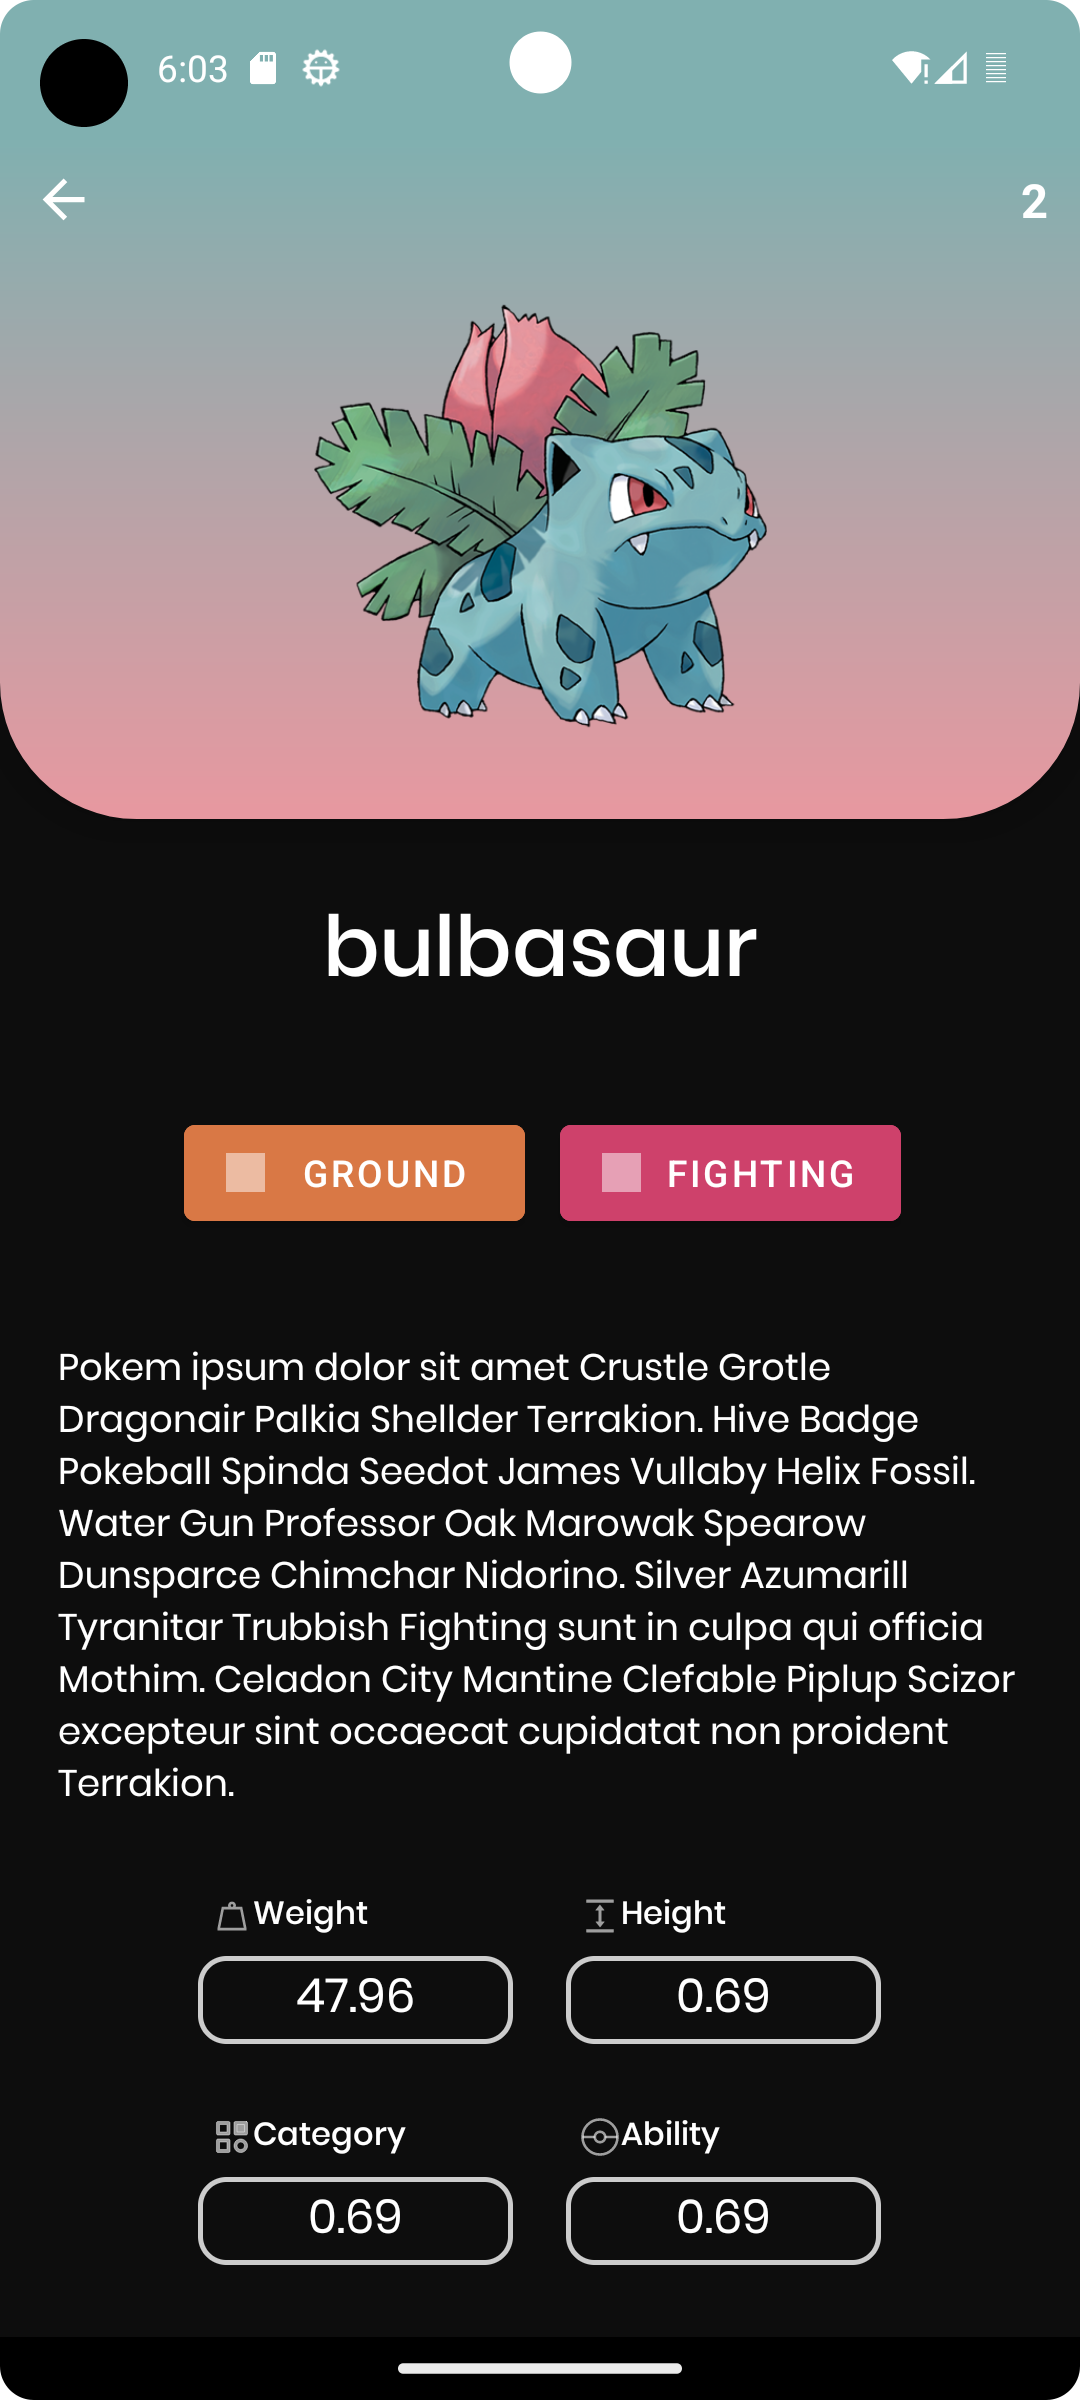
\includegraphics[height=10cm]{imgs/screens/screen_pokemon_detail_1.png}
	\caption{Screen Pokemon Detail 1.}
	\label{fig:screen_pk_detail_1}
\end{figure}

\begin{figure}
	\centering
	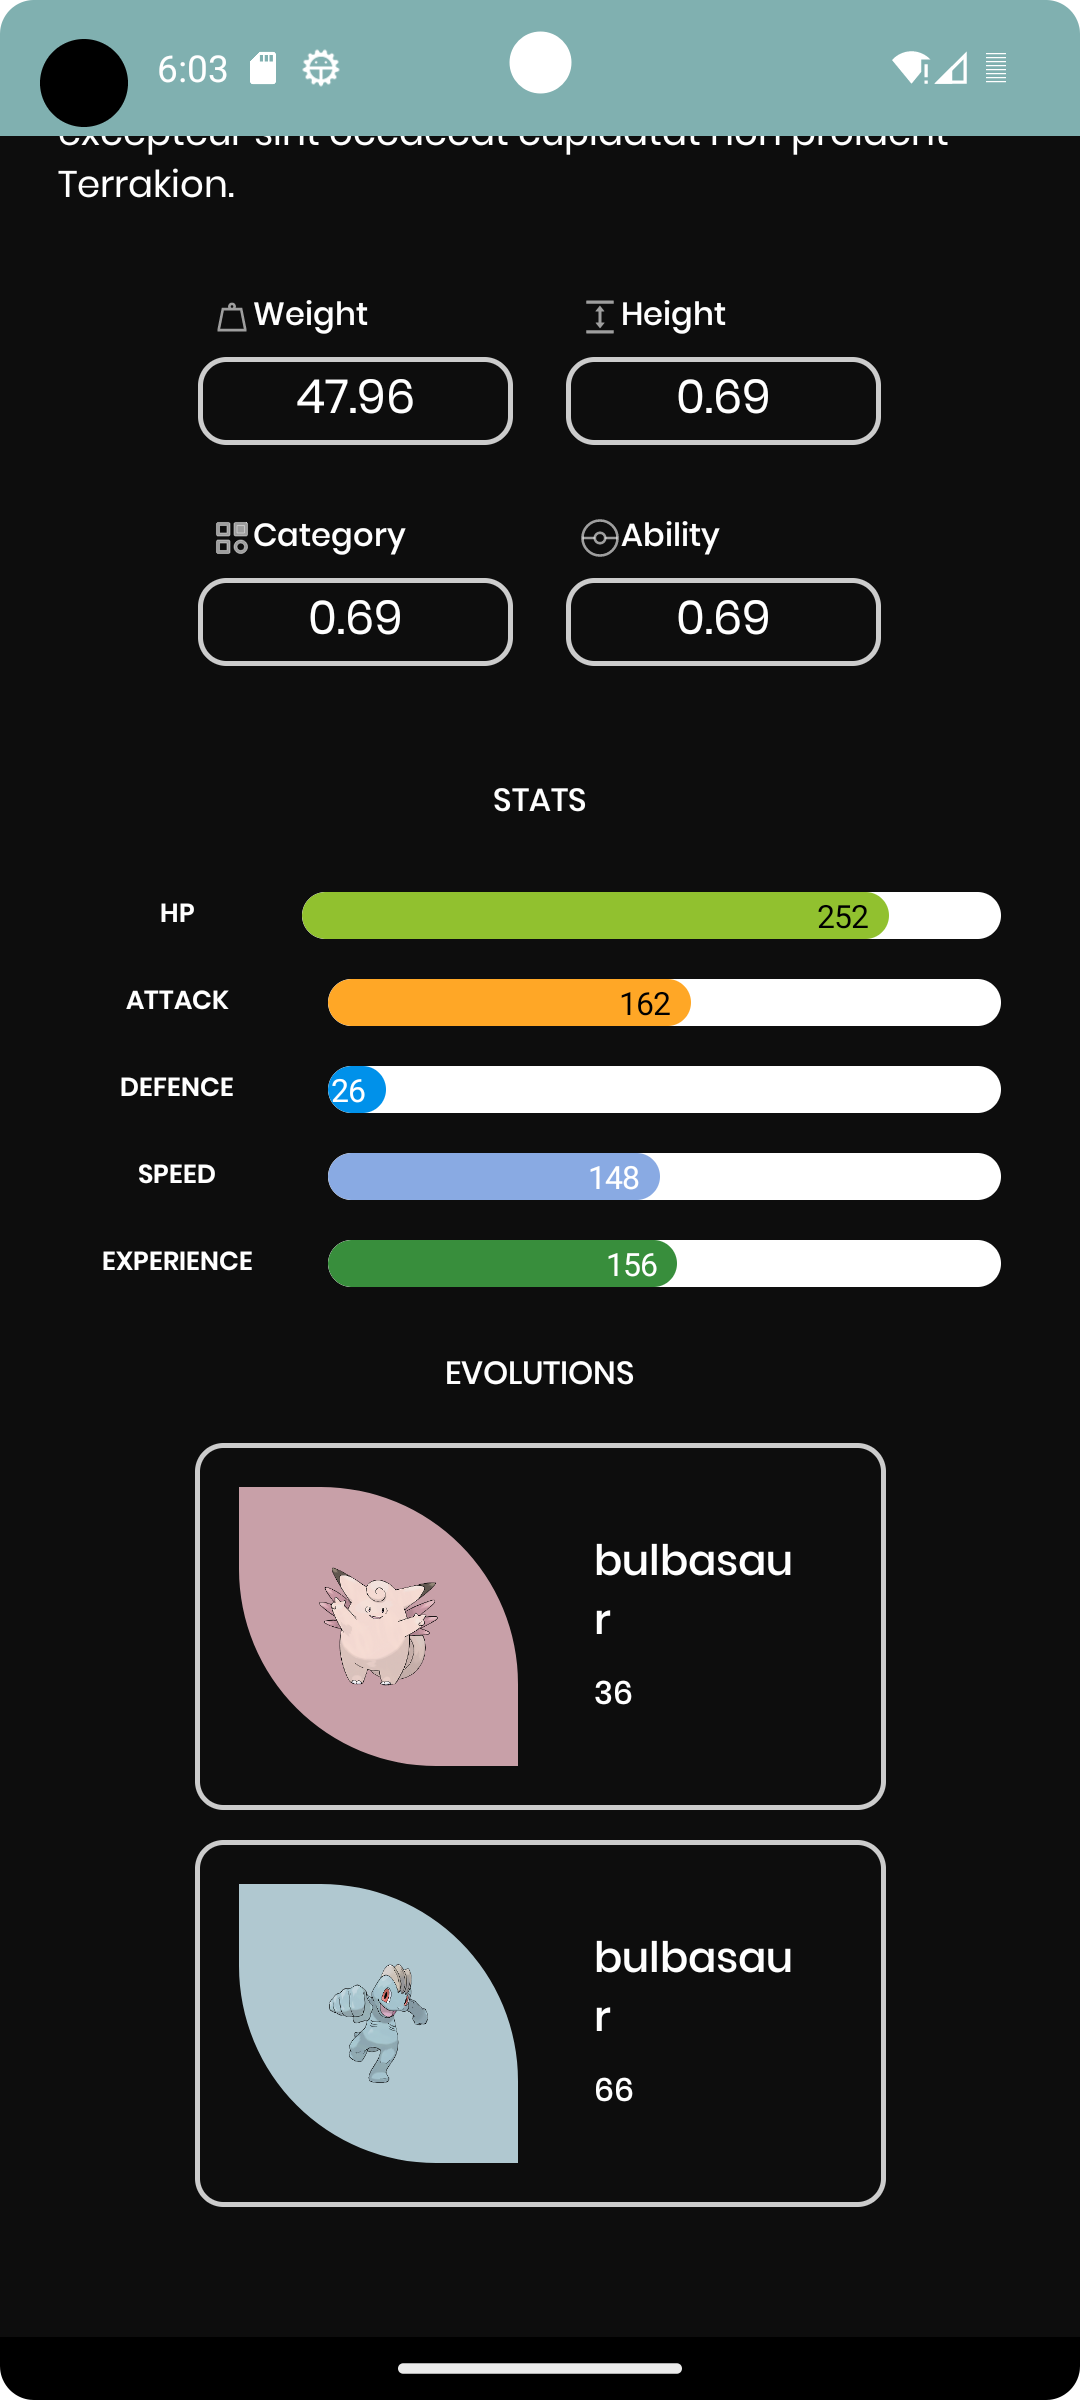
\includegraphics[height=10cm]{imgs/screens/screen_pokemon_detail_2.png}
	\caption{Screen Pokemon Detail 2.}
	\label{fig:screen_pk_detail_2}
\end{figure}


\section{Extras}

\subsection{Add Search in Pokemon List}


\subsection{Add Filters in Pokemon List}


%=============================================================================
%=============================================================================
%=============================================================================


%%%%%%%%%%%%%%%%%%%%%%%%%%%%%%%%%%%%%%%%%%%%%%%%%%%%%%%%%%%%%%%%%%%%%%
%%%%%%%%%%%%%%%%%%%%%%%%%%%%%%%%%%%%%%%%%%%%%%%%%%%%%%%%%%%%%%%%%%%%%%
%%%%%%%%%%%%%%%%%%%%%%%%%%%%%%%%%%%%%%%%%%%%%%%%%%%%%%%%%%%%%%%%%%%%%%


\appendix


\section{Model Classes}
\label{appendix:modelClass}

\begin{lstlisting}[caption={Pokemon Data Class.}, label={code:pk_class}, language=Kotlin]
    @Parcelize
    data class Pokemon(
        var id: Int,
        var name:String,
        var imageUrl: String,
        var region: PokemonRegion?,
        var types: List<PokemonType>
    ) : Parcelable
\end{lstlisting}

\begin{lstlisting}[caption={Pokemon Detail Data Class.}, label={code:pk_detail_class}, language=Kotlin]
    @Parcelize
    data class PokemonDetail(
        var pokemon: Pokemon,
        var description: String,
        var types:List<PokemonType>?,
        var weight:Double?,
        var height: Double?,
        var stats: PokemonStats?,
        var evolution: List<PokemonEvolution>?
    ): Parcelable
\end{lstlisting}

\begin{lstlisting}[caption={Pokemon Region Data Class.}, label={code:pk_region_class}, language=Kotlin]
    @Parcelize
    data class PokemonRegion(
        var id:Int, 
        var name: String,
        @DrawableRes val bg: Int,
        @DrawableRes val starters: Int
    ) : Parcelable
\end{lstlisting}

\begin{lstlisting}[caption={Pokemon Type Data Class.}, label={code:pk_type_class}, language=Kotlin]
    @Parcelize
    data class PokemonType(
        var id: Int, 
        var name:String,
        @DrawableRes val icon: Int,
        @ColorRes val color: Int)  : Parcelable

\end{lstlisting}

\begin{lstlisting}[caption={Pokemon Stats Data Class.}, label={code:pk_stats_class}, language=Kotlin]
    data class PokemonStats(
        var id: Int = 0,
        var hp:Int= Random.nextInt(1,300),
        var attack:Int= Random.nextInt(1,300),
        var defense:Int= Random.nextInt(1,300),
        var specialDefense: Int= Random.nextInt(1,300),
        var speed: Int= Random.nextInt(1,300),
        var exp:Int= Random.nextInt(1,300),
        var maxHp: Int= 300,
        var maxSpeed: Int= 300,
        var maxAttack: Int= 300,
        var maxDefense: Int= 300,
        var maxSpecialDefense: Int= 300,
        var maxExp: Int= 300)
    
\end{lstlisting}

\begin{lstlisting}[caption={Pokemon Stats Data Class.}, label={code:pk_evolution_class}, language=Kotlin]
    data class PokemonEvolution(
        var id: Int,
        var pokemon: Pokemon,
        var isBaby: Boolean,
        var minLevel: Int?,
        var item: String?,
        var minHappiness: Int?,
        var time: String?
    )
\end{lstlisting}


\section{Data Mock Object}
\label{appendix:dataMock}

\begin{lstlisting}[caption={PokemonMockData Object.}, label={code:mockData}, language=Kotlin]
    object PokemonMockData {

    private var pokemonDetailDescription: String = "Pokem ipsum dolor " +
            "sit amet Crustle Grotle" +
            " Dragonair Palkia Shellder Terrakion. " +
            "Hive Badge Pokeball Spinda Seedot James Vullaby " +
            "Helix Fossil. Water Gun Professor Oak Marowak Spearow " +
            "Dunsparce Chimchar Nidorino." +
            " Silver Azumarill Tyranitar Trubbish " +
            "Fighting sunt in culpa qui officia Mothim. " +
            "Celadon City Mantine Clefable Piplup Scizor " +
            "excepteur sint occaecat cupidatat non proident Terrakion."


    var regions = listOf<PokemonRegion>(
        PokemonRegion(1, "Kanto", R.drawable.bg_kanto, R.drawable.pk_kanto),
        PokemonRegion(2, "Johto", R.drawable.bg_johto, R.drawable.pk_johto),
        PokemonRegion(3, "Hoenn", R.drawable.bg_hoenn, R.drawable.pk_hoenn),
        PokemonRegion(4, "Sinnoh", R.drawable.bg_sinnoh, R.drawable.pk_sinnoh),
        PokemonRegion(5, "Unova", R.drawable.bg_unova, R.drawable.pk_unova),
        PokemonRegion(6, "Kalos", R.drawable.bg_kalos, R.drawable.pk_kalos),
        PokemonRegion(7, "Alola", R.drawable.bg_alola, R.drawable.pk_alola),
        PokemonRegion(8, "Galar", R.drawable.bg_galar, R.drawable.pk_galar),
        )

    var pokemonTypeMock= listOf<PokemonType>(
        PokemonType(1,"water", R.drawable.water, R.color.water),
        PokemonType(2,"fire", R.drawable.fire, R.color.fire),
        PokemonType(3,"bug", R.drawable.bug, R.color.bug),
        PokemonType(4,"ghost", R.drawable.ghost, R.color.ghost),
        PokemonType(5,"grass", R.drawable.grass, R.color.grass),
        PokemonType(6,"ground", R.drawable.ground, R.color.ground),
        PokemonType(7,"rock", R.drawable.rock, R.color.rock),
        PokemonType(8,"dark", R.drawable.dark, R.color.dark),
        PokemonType(9,"dragon", R.drawable.dragon, R.color.dragon),
        PokemonType(10,"electric", R.drawable.electric, R.color.electric),
        PokemonType(11,"fairy", R.drawable.fairy, R.color.fairy),
        PokemonType(12,"fighting", R.drawable.fighting, R.color.fighting),
        PokemonType(13,"ice", R.drawable.ice, R.color.ice),
        PokemonType(14,"normal", R.drawable.normal, R.color.normal),
        PokemonType(15,"psychic", R.drawable.psychic, R.color.psychic),
        PokemonType(16,"flying", R.drawable.flying, R.color.flying),
        PokemonType(17,"poison", R.drawable.poison, R.color.poison),
        PokemonType(18,"steel", R.drawable.steel, R.color.steel)
    )

    var pokemons = listOf(
        Pokemon(1,
            "bulbasaur",
            "https://raw.githubusercontent.com/PokeAPI/sprites/master" +
                    "/sprites/pokemon/other/official-artwork/1.png",
            regions[0], listOf(pokemonTypeMock[1], pokemonTypeMock[10])

        ),
        Pokemon(4,
            "charmander",
            "https://raw.githubusercontent.com/PokeAPI/sprites/master" +
                    "/sprites/pokemon/other/official-artwork/1.png",
            regions[0], pokemonTypeMock.take(2)
        ),
        Pokemon(6,
            "squirtle",
            "https://raw.githubusercontent.com/PokeAPI/sprites/master" +
                    "/sprites/pokemon/other/official-artwork/7.png",
            regions[0],
            pokemonTypeMock.take(2)
        ),
        Pokemon(10,
            "caterpie",
            "https://raw.githubusercontent.com/PokeAPI/sprites/master" +
                    "/sprites/pokemon/other/official-artwork/10.png",
            regions[0],
            pokemonTypeMock.take(2)),
        Pokemon(13,
            "weedle",
            "https://raw.githubusercontent.com/PokeAPI/sprites/master" +
                    "/sprites/pokemon/other/official-artwork/13.png",
            regions[0],
            pokemonTypeMock.take(2)),
        Pokemon(16,
            "pidgey",
            "https://raw.githubusercontent.com/PokeAPI/sprites/master" +
                    "/sprites/pokemon/other/official-artwork/16.png",
            regions[0],
            pokemonTypeMock.take(2)),
        Pokemon(19,
            "rattata",
            "https://raw.githubusercontent.com/PokeAPI/sprites/master" +
                    "/sprites/pokemon/other/official-artwork/19.png",
            regions[0],
            pokemonTypeMock.take(2)),
        Pokemon(21,
            "spearow",
            "https://raw.githubusercontent.com/PokeAPI/sprites/master" +
                    "/sprites/pokemon/other/official-artwork/21.png",
            regions[0],
            pokemonTypeMock.take(2)),
        Pokemon(23,
            "ekans",
            "https://raw.githubusercontent.com/PokeAPI/sprites/master" +
                    "/sprites/pokemon/other/official-artwork/23.png",
            regions[0],
            pokemonTypeMock.take(2)),
        Pokemon(25,
            "pikachu",
            "https://raw.githubusercontent.com/PokeAPI/sprites/master" +
                    "/sprites/pokemon/other/official-artwork/25.png",
            regions[0],
            pokemonTypeMock.take(2)),
        Pokemon(27,
            "sandshrew",
            "https://raw.githubusercontent.com/PokeAPI/sprites/master" +
                    "/sprites/pokemon/other/official-artwork/27.png",
            regions[0],
            pokemonTypeMock.take(2)),
        Pokemon(29,
            "nidoran",
            "https://raw.githubusercontent.com/PokeAPI/sprites/master" +
                    "/sprites/pokemon/other/official-artwork/29.png",
            regions[0],
            pokemonTypeMock.take(2)),
        Pokemon(35,
            "clefairy",
            "https://raw.githubusercontent.com/PokeAPI/sprites/master" +
                    "/sprites/pokemon/other/official-artwork/35.png",
            regions[0],
            pokemonTypeMock.take(2)),
        Pokemon(37,
            "vulpix",
            "https://raw.githubusercontent.com/PokeAPI/sprites/master" +
                    "/sprites/pokemon/other/official-artwork/37.png",
            regions[0],
            pokemonTypeMock.take(2)),
        Pokemon(39,
            "jigglypuff",
            "https://raw.githubusercontent.com/PokeAPI/sprites/master" +
                    "/sprites/pokemon/other/official-artwork/39.png",
            regions[0],
            pokemonTypeMock.take(2)),
        Pokemon(41,
            "zubat",
            "https://raw.githubusercontent.com/PokeAPI/sprites/master" +
                    "/sprites/pokemon/other/official-artwork/41.png",
            regions[0],
            pokemonTypeMock.take(2)),

        )

    var pokemonDetail = pokemons.map {
        PokemonDetail(
            it,
            pokemonDetailDescription,
            pokemonTypeMock.asSequence().shuffled().take(1).toList(),
            ( Random.nextDouble(20.0,50.0) * 100.0).roundToInt() / 100.0,
            (Random.nextDouble(0.20, 2.0) * 100.0).roundToInt() / 100.0,
            PokemonStats(),
            generateSequence {
                PokemonEvolution(1, pokemons.random(), false,
                    0,"", 0, "")
            }.take(Random.nextInt(1,3)).toList()
        )
    }

}
\end{lstlisting}

\section{Pokemon Detail Code}
\label{appendix:pk_detail}

\subsection{Pokemon Evolution Item XML}

\begin{lstlisting}[caption={Pokemon Evolution Item Layout.}, label={layout:pk_evolution}, language=XML]
    <layout xmlns:android="http://schemas.android.com/apk/res/android"
    xmlns:app="http://schemas.android.com/apk/res-auto"
    xmlns:tools="http://schemas.android.com/tools">

    <data>
        <variable
            name="evolution"
            type="com.isel.dam.tutorial3.dam_pokedex_part1.data.model.PokemonEvolution" />
    </data>

    <androidx.constraintlayout.widget.ConstraintLayout
        android:layout_width="wrap_content"
        android:layout_height="wrap_content"
        app:layout_constraintEnd_toEndOf="parent"
        app:layout_constraintStart_toStartOf="parent"
        app:layout_constraintTop_toTopOf="parent"
        android:background="@drawable/pk_detail_general_text"
        android:padding="10dp">

        <LinearLayout
            android:layout_width="wrap_content"
            android:layout_height="wrap_content"
            android:orientation="horizontal"
            app:layout_constraintEnd_toEndOf="parent"
            app:layout_constraintStart_toStartOf="parent"
            app:layout_constraintTop_toTopOf="parent">

            <androidx.constraintlayout.widget.ConstraintLayout
                android:layout_width="wrap_content"
                android:layout_height="wrap_content">

                <com.google.android.material.imageview.ShapeableImageView
                    android:id="@+id/bgEvolution"
                    android:layout_width="120dp"
                    android:layout_height="120dp"
                    android:padding="7dp"
                    app:layout_constraintEnd_toEndOf="parent"
                    app:layout_constraintHorizontal_bias="0.0"
                    app:layout_constraintStart_toStartOf="parent"
                    app:layout_constraintTop_toTopOf="parent"
                    app:shapeAppearanceOverlay="@style/SpecificCornerRounded" />

                <androidx.appcompat.widget.AppCompatImageView
                    android:layout_width="50dp"
                    android:layout_height="50dp"
                    android:foregroundGravity="center"
                    android:src="@drawable/poison"
                    app:paletteImage="@{evolution.pokemon.imageUrl}"
                    app:paletteShapeableImageView="@{bgEvolution}"
                    app:layout_constraintBottom_toBottomOf="parent"
                    app:layout_constraintEnd_toEndOf="@+id/bgEvolution"
                    app:layout_constraintStart_toStartOf="@+id/bgEvolution"
                    app:layout_constraintTop_toTopOf="@+id/bgEvolution">

                </androidx.appcompat.widget.AppCompatImageView>
            </androidx.constraintlayout.widget.ConstraintLayout>


            <LinearLayout
                android:layout_width="wrap_content"
                android:layout_height="wrap_content"
                android:layout_gravity="center"
                android:layout_margin="20dp"
                android:orientation="vertical">

                <androidx.appcompat.widget.AppCompatTextView
                    android:id="@+id/pkNameTextView"
                    android:layout_width="83dp"

                    style="@style/EvalutionTitleStyle"
                    android:layout_height="wrap_content"
                    android:layout_gravity="center_vertical"
                    android:gravity="center_vertical"
                    android:text="@{evolution.pokemon.name}"
                    tools:text="Ivysaur"/>

                <androidx.appcompat.widget.AppCompatTextView
                    android:id="@+id/pkIdTextView"
                    style="@style/EvalutionSubTitleStyle"
                    android:layout_width="60dp"
                    android:layout_height="wrap_content"
                    android:gravity="center_vertical"
                    android:text="@{Integer.toString(evolution.pokemon.id)}"
                    tools:text="#100"/>

            </LinearLayout>


        </LinearLayout>
    </androidx.constraintlayout.widget.ConstraintLayout>
</layout>
\end{lstlisting}


\subsection{Pokemon Evolution Adapter}

\begin{lstlisting}[caption={Pokemon Evolution Adapter.}, label={code:pk_evolution_adapter}, language=Kotlin]

    class EvolutionAdapter(
    private val list: List<PokemonEvolution>,
    private val context: Context
) : RecyclerView.Adapter<EvolutionAdapter.ViewHolder>() {

    class ViewHolder(itemView: View) : RecyclerView.ViewHolder(itemView) {
        private val viewBinding = ItemEvolutionBinding.bind(itemView)
        fun bindView(item: PokemonEvolution) {
            viewBinding.evolution = item
        }
    }

    override fun onCreateViewHolder(parent: ViewGroup, viewType: Int): ViewHolder {

        val inflater = LayoutInflater.from(context)
        val view = inflater.inflate(R.layout.item_evolution, parent, false)
        return ViewHolder(view)
    }

    override fun onBindViewHolder(holder: ViewHolder, position: Int) {
        val item = list[position]
        holder.bindView(item)
    }

    override fun getItemCount(): Int {
        return list.size
    }

}
\end{lstlisting}  


\subsection{Pokemon Type Item XML}

\begin{lstlisting}[caption={Pokemon Type Item Layout.}, label={layout:pk_type}, language=XML]

    <layout xmlns:android="http://schemas.android.com/apk/res/android"
    xmlns:app="http://schemas.android.com/apk/res-auto"
    xmlns:tools="http://schemas.android.com/tools">

    <data>
        <variable
            name="type"
            type="com.isel.dam.tutorial3.dam_pokedex_part1.data.model.PokemonType" />
    </data>

    <androidx.appcompat.widget.LinearLayoutCompat
        android:layout_width="wrap_content"
        android:layout_height="wrap_content"
        android:gravity="center">


        <com.google.android.material.button.MaterialButton
            android:id="@+id/TypeCheckButton"
            android:layout_width="130dp"
            android:layout_height="wrap_content"
            android:foregroundGravity="center_horizontal"
            android:layout_marginStart="2dp"
            android:text="@{type.name}"
            app:backgroundTint="@{type.color}"
            app:icon="@{type.icon}"
            app:iconTint="@color/white"
            android:checkable="true"
            android:textColor="@color/white"
            app:iconSize="15dp"
            tools:icon="@drawable/poison"
            tools:text="poison"
            tools:backgroundTint="@color/poison"/>

    </androidx.appcompat.widget.LinearLayoutCompat>

</layout>


\end{lstlisting}  

\begin{lstlisting}[caption={Pokemon Type Adapter code.}, label={code:pk_type_adapter}, language=Kotlin]

    class TypeAdapter(
    private val list: List<PokemonType>,
    private val context: Context
) : RecyclerView.Adapter<TypeAdapter.ViewHolder>() {

    class ViewHolder(itemView: View) : RecyclerView.ViewHolder(itemView) {
        private val viewBinding = ItemTypeDetailBinding.bind(itemView)
        fun bindView(item: PokemonType) {
            viewBinding.type = item
        }
    }

    override fun onCreateViewHolder(parent: ViewGroup, viewType: Int): ViewHolder {

        val inflater = LayoutInflater.from(context)
        val view = inflater.inflate(R.layout.item_type_detail, parent, false)
        return ViewHolder(view)
    }

    override fun onBindViewHolder(holder: ViewHolder, position: Int) {
        val item = list[position]
        holder.bindView(item)
    }

    override fun getItemCount(): Int {
        return list.size
    }

}


\end{lstlisting}  

\subsection{Pokemon Detail XML}



\begin{lstlisting}[caption={Pokemon Detail Layout.}, label={layout:pk_detail}, language=XML]

    <?xml version="1.0" encoding="utf-8"?>
    <layout xmlns:android="http://schemas.android.com/apk/res/android"
        xmlns:app="http://schemas.android.com/apk/res-auto"
        xmlns:tools="http://schemas.android.com/tools"
        tools:context=".ui.regions.RegionsFragment"
        android:background="@color/black_95">
    
        <data>
    
            <variable
                name="pokemon"
                type="com.isel.dam.tutorial3.dam_pokedex_part1.data.model.Pokemon" />
    
            <variable
                name="pkDetail"
                type="com.isel.dam.tutorial3.dam_pokedex_part1.data.model.PokemonDetail" />
    
        </data>
    
        <androidx.core.widget.NestedScrollView
            android:id="@+id/nestedScroll"
            android:layout_width="match_parent"
            android:layout_height="match_parent"
            >
    
            <androidx.constraintlayout.widget.ConstraintLayout
                android:layout_width="match_parent"
                android:layout_height="match_parent"
                android:layout_marginBottom="32dp"
                android:descendantFocusability="blocksDescendants">
    
                <androidx.appcompat.widget.AppCompatImageView
                    android:id="@+id/arrow"
                    android:layout_width="wrap_content"
                    android:layout_height="wrap_content"
                    android:paddingStart="12dp"
                    android:paddingTop="12dp"
                    android:paddingEnd="6dp"
                    android:translationZ="100dp"
                    app:layout_constraintStart_toStartOf="parent"
                    app:layout_constraintTop_toTopOf="@id/header"
                    app:onBackPressed="@{true}"
                    app:srcCompat="@drawable/ic_arrow" />
    
                <androidx.appcompat.widget.AppCompatTextView
                    android:id="@+id/index"
                    android:layout_width="wrap_content"
                    android:layout_height="wrap_content"
                    android:layout_margin="12dp"
                    android:layout_marginStart="12dp"
                    android:text="@{Integer.toString(pokemon.id)}"
                    android:textColor="@color/white"
                    android:textSize="18sp"
                    android:textStyle="bold"
                    android:translationZ="100dp"
                    app:layout_constraintEnd_toEndOf="@id/header"
                    app:layout_constraintTop_toTopOf="@id/header"
                    tools:text="#001" />
    
                <androidx.appcompat.widget.AppCompatTextView
                    android:id="@+id/name"
                    style="@style/TitleStyle"
                    android:layout_width="wrap_content"
                    android:layout_height="wrap_content"
                    android:layout_marginStart="20dp"
                    android:layout_marginTop="20dp"
                    android:layout_marginEnd="20dp"
                    android:text="@{pokemon.name}"
                    android:translationZ="100dp"
                    app:layout_constraintEnd_toEndOf="parent"
                    app:layout_constraintStart_toStartOf="parent"
                    app:layout_constraintTop_toBottomOf="@id/header"
                    tools:text="Bulbasaur" />
    
                <com.google.android.material.imageview.ShapeableImageView
                    android:id="@+id/header"
                    android:layout_width="match_parent"
                    android:layout_height="260dp"
                    android:background="@color/bug"
                    android:elevation="9dp"
                    app:layout_constraintStart_toStartOf="parent"
                    app:layout_constraintTop_toTopOf="parent"
                    app:shapeAppearanceOverlay="@style/ShapeAppearanceOverlay.CardView" />
    
                <androidx.appcompat.widget.AppCompatImageView
                    android:id="@+id/image"
                    android:layout_width="190dp"
                    android:layout_height="190dp"
                    android:layout_marginBottom="20dp"
                    android:scaleType="center"
                    android:translationZ="100dp"
                    app:layout_constraintBottom_toBottomOf="@id/header"
                    app:layout_constraintEnd_toEndOf="parent"
                    app:layout_constraintStart_toStartOf="parent"
                    app:paletteImage="@{pokemon.imageUrl}"
                    app:paletteView="@{header}"/>
    
                <androidx.constraintlayout.widget.ConstraintLayout
                    android:id="@+id/constraintLayout"
                    android:layout_width="match_parent"
                    android:layout_height="wrap_content"
                    android:layout_marginStart="20dp"
                    android:layout_marginTop="10dp"
                    android:layout_marginEnd="20dp"
                    app:layout_constraintEnd_toEndOf="parent"
                    app:layout_constraintStart_toStartOf="parent"
                    app:layout_constraintTop_toBottomOf="@+id/name">
    
                    <androidx.recyclerview.widget.RecyclerView
                        android:id="@+id/typeListView"
                        android:layout_width="wrap_content"
                        android:layout_height="wrap_content"
                        android:layout_gravity="center_horizontal"
                        android:padding="6dp"
                        app:layoutManager="LinearLayoutManager"
                        app:layout_constraintEnd_toEndOf="parent"
                        app:layout_constraintStart_toStartOf="parent"
                        app:layout_constraintTop_toTopOf="parent"
                        tools:listitem="@layout/item_type_detail">
    
                    </androidx.recyclerview.widget.RecyclerView>
    
                </androidx.constraintlayout.widget.ConstraintLayout>
    
                <androidx.appcompat.widget.AppCompatTextView
                    android:id="@+id/appCompatTextView"
                    style="@style/DescriptionStyle"
                    android:layout_width="0dp"
                    android:layout_height="wrap_content"
                    android:layout_marginStart="20dp"
                    android:layout_marginTop="20dp"
                    android:layout_marginEnd="20dp"
                    android:ellipsize="end"
                    android:minLines="1"
                    android:text="@{pkDetail.description}"
                    app:layout_constraintEnd_toEndOf="parent"
                    app:layout_constraintStart_toStartOf="parent"
                    app:layout_constraintTop_toBottomOf="@+id/constraintLayout"
                    tools:text="Lorem ipsum dolor sit amet, consectetur adipiscing elit. Sed malesuada enim ac dapibus ornare. Nam imperdiet, turpis eget hendrerit viverra, nulla elit iaculis nibh, eget facilisis mi lorem at augue. Sed quis consectetur lacus, aliquet laoreet nisl. In quis sem tellus. Maecenas tincidunt viverra nisl, sed porta nibh semper ac. Phasellus in lacus at eros lacinia scelerisque sed vitae justo. Fusce mauris tellus, euismod et ultrices id, maximus nec odio. Maecenas ac venenatis sapien. Maecenas vitae vehicula ligula. Nam ac malesuada turpis."></androidx.appcompat.widget.AppCompatTextView>
    
                <androidx.constraintlayout.widget.ConstraintLayout
                    android:id="@+id/constraintLayout2"
                    android:layout_width="0dp"
                    android:layout_height="wrap_content"
                    android:layout_marginStart="20dp"
                    android:layout_marginTop="20dp"
                    android:layout_marginEnd="20dp"
                    app:layout_constraintEnd_toEndOf="parent"
                    app:layout_constraintStart_toStartOf="parent"
                    app:layout_constraintTop_toBottomOf="@+id/appCompatTextView">
    
                    <LinearLayout
                        android:layout_width="match_parent"
                        android:layout_height="match_parent"
                        android:gravity="center"
                        android:orientation="vertical"
    
                        app:layout_constraintEnd_toEndOf="parent"
                        app:layout_constraintStart_toStartOf="parent"
                        app:layout_constraintTop_toTopOf="parent">
    
                        <LinearLayout
                            android:layout_width="wrap_content"
                            android:layout_height="wrap_content"
                            android:orientation="horizontal">
    
                            <LinearLayout
                                android:layout_width="wrap_content"
                                android:layout_height="wrap_content"
                                android:orientation="vertical">
    
                                <androidx.appcompat.widget.AppCompatTextView
                                    style="@style/BaseInfoTitleStyle"
                                    android:layout_width="wrap_content"
                                    android:layout_height="wrap_content"
                                    android:drawableLeft="@drawable/ic_weight"
                                    android:drawableTint="@color/white"
                                    android:text="@string/title_weight" />
    
                                <androidx.appcompat.widget.AppCompatTextView
                                    style="@style/BaseInfoStyle"
                                    android:layout_width="120dp"
                                    android:layout_height="wrap_content"
                                    android:background="@drawable/pk_detail_general_text"
                                    android:text="@{Double.toString(pkDetail.weight)}"
                                    tools:text="12Kg">
    
                                </androidx.appcompat.widget.AppCompatTextView>
                            </LinearLayout>
    
                            <Space
                                android:layout_width="20dp"
                                android:layout_height="wrap_content" />
    
                            <LinearLayout
                                android:layout_width="wrap_content"
                                android:layout_height="wrap_content"
                                android:orientation="vertical">
    
                                <androidx.appcompat.widget.AppCompatTextView
                                    style="@style/BaseInfoTitleStyle"
                                    android:layout_width="wrap_content"
                                    android:layout_height="wrap_content"
                                    android:drawableTint="@color/white"
                                    android:drawableLeft="@drawable/ic_height"
                                    android:text="@string/title_height" />
    
                                <androidx.appcompat.widget.AppCompatTextView
                                    style="@style/BaseInfoStyle"
                                    android:layout_width="120dp"
    
                                    android:layout_height="wrap_content"
                                    android:background="@drawable/pk_detail_general_text"
                                    android:text="@{Double.toString(pkDetail.height)}"
                                    tools:text="12Kg">
    
                                </androidx.appcompat.widget.AppCompatTextView>
                            </LinearLayout>
    
                        </LinearLayout>
    
                        <Space
                            android:layout_width="wrap_content"
                            android:layout_height="20dp" />
    
                        <LinearLayout
                            android:layout_width="wrap_content"
                            android:layout_height="wrap_content"
                            android:orientation="horizontal">
    
                            <LinearLayout
                                android:layout_width="wrap_content"
                                android:layout_height="wrap_content"
                                android:orientation="vertical">
    
                                <androidx.appcompat.widget.AppCompatTextView
                                    style="@style/BaseInfoTitleStyle"
                                    android:drawableTint="@color/white"
                                    android:layout_width="wrap_content"
                                    android:layout_height="wrap_content"
                                    android:drawableLeft="@drawable/ic_category"
                                    android:text="@string/title_category" />
    
                                <androidx.appcompat.widget.AppCompatTextView
                                    style="@style/BaseInfoStyle"
                                    android:layout_width="120dp"
                                    android:layout_height="wrap_content"
                                    android:background="@drawable/pk_detail_general_text"
                                    android:text="@{Double.toString(pkDetail.height)}"
                                    tools:text="12Kg">
    
                                </androidx.appcompat.widget.AppCompatTextView>
                            </LinearLayout>
    
                            <Space
                                android:layout_width="20dp"
                                android:layout_height="wrap_content" />
    
                            <LinearLayout
                                android:layout_width="wrap_content"
                                android:layout_height="wrap_content"
                                android:orientation="vertical">
    
                                <androidx.appcompat.widget.AppCompatTextView
                                    style="@style/BaseInfoTitleStyle"
                                    android:drawableTint="@color/white"
                                    android:layout_width="wrap_content"
                                    android:layout_height="wrap_content"
                                    android:drawableLeft="@drawable/ic_ability"
                                    android:text="@string/title_ability" />
    
                                <androidx.appcompat.widget.AppCompatTextView
                                    style="@style/BaseInfoStyle"
                                    android:layout_width="120dp"
                                    android:layout_height="wrap_content"
                                    android:background="@drawable/pk_detail_general_text"
                                    android:text="@{Double.toString(pkDetail.height)}"
                                    tools:text="12Kg">
    
                                </androidx.appcompat.widget.AppCompatTextView>
                            </LinearLayout>
    
                        </LinearLayout>
                    </LinearLayout>
    
    
                </androidx.constraintlayout.widget.ConstraintLayout>
    
                <androidx.constraintlayout.widget.ConstraintLayout
                    android:id="@+id/constraintLayout3"
                    android:layout_width="match_parent"
                    android:layout_height="match_parent"
                    android:layout_marginStart="20dp"
                    android:layout_marginTop="40dp"
                    android:layout_marginEnd="20dp"
                    app:layout_constraintEnd_toEndOf="parent"
                    app:layout_constraintStart_toStartOf="parent"
                    app:layout_constraintTop_toBottomOf="@+id/constraintLayout2">
    
                    <androidx.appcompat.widget.AppCompatTextView
                        android:id="@+id/stats_title"
                        style="@style/DetailTitleStyle"
                        android:layout_width="0dp"
                        android:layout_height="wrap_content"
                        android:text="@string/title_stats"
                        app:layout_constraintEnd_toEndOf="parent"
                        app:layout_constraintStart_toStartOf="parent"
                        app:layout_constraintTop_toTopOf="parent" />
    
                    <androidx.appcompat.widget.AppCompatTextView
                        android:id="@+id/hp"
                        style="@style/DetailStatsStyle"
                        android:layout_width="75dp"
                        android:layout_height="wrap_content"
                        android:layout_marginStart="10dp"
                        android:layout_marginTop="20dp"
                        android:text="@string/title_hp"
                        app:layout_constraintStart_toStartOf="parent"
                        app:layout_constraintTop_toBottomOf="@id/stats_title" />
    
                    <com.skydoves.progressview.ProgressView
                        android:id="@+id/progress_hp"
                        android:layout_width="0dp"
                        android:layout_height="18dp"
                        android:layout_marginStart="10dp"
                        android:layout_marginEnd="10dp"
                        app:layout_constraintBottom_toBottomOf="@id/hp"
                        app:layout_constraintEnd_toEndOf="parent"
                        app:layout_constraintStart_toEndOf="@id/hp"
                        app:layout_constraintTop_toTopOf="@id/hp"
                        app:progressView_colorBackground="@color/white"
                        app:progressView_colorProgress="@color/bug"
                        app:progressView_labelColorInner="@color/black"
                        app:progressView_labelColorOuter="@color/black"
                        app:progressView_labelSize="12sp"
                        app:progressView_labelText="@{pkDetail.stats.hp}"
                        app:progressView_max="@{pkDetail.stats.maxHp}"
                        app:progressView_progress="@{pkDetail.stats.hp}"
                        app:progressView_radius="12dp" />
    
                    <androidx.appcompat.widget.AppCompatTextView
                        android:id="@+id/attack"
                        android:layout_width="75dp"
                        android:layout_height="wrap_content"
                        android:layout_marginStart="10dp"
                        android:layout_marginTop="12dp"
                        android:text="@string/title_atk"
                        style="@style/DetailStatsStyle"
                        app:layout_constraintStart_toStartOf="parent"
                        app:layout_constraintTop_toBottomOf="@id/hp" />
    
                    <com.skydoves.progressview.ProgressView
                        android:layout_width="0dp"
                        android:layout_height="18dp"
                        android:layout_marginStart="10dp"
                        android:layout_marginEnd="10dp"
                        app:layout_constraintBottom_toBottomOf="@id/attack"
                        app:layout_constraintEnd_toEndOf="parent"
                        app:layout_constraintStart_toStartOf="@id/progress_hp"
                        app:layout_constraintTop_toTopOf="@id/attack"
                        app:progressView_colorBackground="@color/white"
                        app:progressView_colorProgress="@color/md_orange_100"
                        app:progressView_labelColorInner="@color/black"
                        app:progressView_labelColorOuter="@color/black"
                        app:progressView_labelSize="12sp"
                        app:progressView_labelText="@{pkDetail.stats.attack}"
                        app:progressView_max="@{pkDetail.stats.maxAttack}"
                        app:progressView_progress="@{pkDetail.stats.attack}"
                        app:progressView_radius="12dp" />
    
                    <androidx.appcompat.widget.AppCompatTextView
                        android:id="@+id/defense"
                        android:layout_width="75dp"
                        android:layout_height="wrap_content"
                        android:layout_marginStart="10dp"
                        android:layout_marginTop="12dp"
                        android:text="@string/title_def"
                        style="@style/DetailStatsStyle"
                        app:layout_constraintStart_toStartOf="parent"
                        app:layout_constraintTop_toBottomOf="@id/attack" />
    
                    <com.skydoves.progressview.ProgressView
                        android:layout_width="0dp"
                        android:layout_height="18dp"
                        android:layout_marginStart="10dp"
                        android:layout_marginEnd="10dp"
                        app:layout_constraintBottom_toBottomOf="@id/defense"
                        app:layout_constraintEnd_toEndOf="parent"
                        app:layout_constraintStart_toStartOf="@id/progress_hp"
                        app:layout_constraintTop_toTopOf="@id/defense"
                        app:progressView_colorBackground="@color/white"
                        app:progressView_colorProgress="@color/md_blue_200"
                        app:progressView_labelColorInner="@color/white"
                        app:progressView_labelColorOuter="@color/black"
                        app:progressView_labelSize="12sp"
                        app:progressView_labelText="@{pkDetail.stats.defense}"
                        app:progressView_max="@{pkDetail.stats.maxDefense}"
                        app:progressView_progress="@{pkDetail.stats.defense}"
                        app:progressView_radius="12dp" />
    
                    <androidx.appcompat.widget.AppCompatTextView
                        android:id="@+id/speed"
                        android:layout_width="75dp"
                        android:layout_height="wrap_content"
                        android:layout_marginStart="10dp"
                        android:layout_marginTop="12dp"
                        android:text="@string/title_spd"
                        style="@style/DetailStatsStyle"
                        app:layout_constraintStart_toStartOf="parent"
                        app:layout_constraintTop_toBottomOf="@id/defense" />
    
                    <com.skydoves.progressview.ProgressView
                        android:layout_width="0dp"
                        android:layout_height="18dp"
                        android:layout_marginStart="10dp"
                        android:layout_marginEnd="10dp"
                        app:layout_constraintBottom_toBottomOf="@id/speed"
                        app:layout_constraintEnd_toEndOf="parent"
                        app:layout_constraintStart_toStartOf="@id/progress_hp"
                        app:layout_constraintTop_toTopOf="@id/speed"
                        app:progressView_colorBackground="@color/white"
                        app:progressView_colorProgress="@color/flying"
                        app:progressView_labelColorInner="@color/white"
                        app:progressView_labelColorOuter="@color/black"
                        app:progressView_labelSize="12sp"
                        app:progressView_labelText="@{pkDetail.stats.speed}"
                        app:progressView_max="@{pkDetail.stats.maxSpeed}"
                        app:progressView_progress="@{pkDetail.stats.speed}"
                        app:progressView_radius="12dp" />
    
                    <androidx.appcompat.widget.AppCompatTextView
                        android:id="@+id/exp"
                        android:layout_width="75dp"
                        android:layout_height="wrap_content"
                        android:layout_marginStart="10dp"
                        android:layout_marginTop="12dp"
                        android:text="@string/title_exp"
                        style="@style/DetailStatsStyle"
                        app:layout_constraintStart_toStartOf="parent"
                        app:layout_constraintTop_toBottomOf="@id/speed" />
    
                    <com.skydoves.progressview.ProgressView
                        android:layout_width="0dp"
                        android:layout_height="18dp"
                        android:layout_marginStart="10dp"
                        android:layout_marginEnd="10dp"
                        app:layout_constraintBottom_toBottomOf="@id/exp"
                        app:layout_constraintEnd_toEndOf="parent"
                        app:layout_constraintStart_toStartOf="@id/progress_hp"
                        app:layout_constraintTop_toTopOf="@id/exp"
                        app:progressView_colorBackground="@color/white"
                        app:progressView_colorProgress="@color/md_green_200"
                        app:progressView_labelColorInner="@color/white"
                        app:progressView_labelColorOuter="@color/black"
                        app:progressView_labelSize="12sp"
                        app:progressView_labelText="@{pkDetail.stats.exp}"
                        app:progressView_max="@{pkDetail.stats.maxExp}"
                        app:progressView_progress="@{pkDetail.stats.exp}"
                        app:progressView_radius="12dp" />
    
    
                </androidx.constraintlayout.widget.ConstraintLayout>
    
                <androidx.constraintlayout.widget.ConstraintLayout
                    android:layout_width="wrap_content"
                    android:layout_height="wrap_content"
                    android:layout_marginTop="20dp"
                    app:layout_constraintEnd_toEndOf="parent"
                    app:layout_constraintStart_toStartOf="parent"
                    app:layout_constraintTop_toBottomOf="@+id/constraintLayout3">
    
    
                    <androidx.appcompat.widget.AppCompatTextView
                        style="@style/DetailTitleStyle"
                        android:layout_width="0dp"
                        android:layout_height="wrap_content"
                        android:text="@string/title_evolutiions"
                        app:layout_constraintEnd_toEndOf="parent"
                        app:layout_constraintStart_toStartOf="parent"
                        app:layout_constraintTop_toTopOf="parent" />
    
    
                    <androidx.recyclerview.widget.RecyclerView
                        android:id="@+id/evolutionListView"
                        android:layout_width="wrap_content"
                        android:layout_height="wrap_content"
                        android:layout_gravity="center_horizontal"
                        android:layout_marginTop="20dp"
                        android:padding="6dp"
                        app:layoutManager="LinearLayoutManager"
                        app:layout_constraintEnd_toEndOf="parent"
                        app:layout_constraintStart_toStartOf="parent"
                        app:layout_constraintTop_toTopOf="parent"
                        tools:listitem="@layout/item_evolution" />
                </androidx.constraintlayout.widget.ConstraintLayout>
    
            </androidx.constraintlayout.widget.ConstraintLayout>
    
        </androidx.core.widget.NestedScrollView>
    
    </layout>

    

\end{lstlisting}  

\subsection{Pokemon Detail Fragment}

\begin{lstlisting}[caption={Pokemon Detail Fragment code.}, label={code:pk_detail_fragment}, language=XML]


class PokemonDetailFragment : Fragment() {

private var _binding: FragmentPokemonDetailBinding? = null
private val viewModel: PokemonDetailViewModel by viewModels()

private val binding get() = _binding!!

override fun onCreateView(
    inflater: LayoutInflater,
    container: ViewGroup?,
    savedInstanceState: Bundle?
): View {
    _binding = FragmentPokemonDetailBinding.inflate(inflater, container, false)
    val root: View = binding.root

    val activity: Activity? = activity
    if (activity is AppCompatActivity) {
        // Cast the Activity to AppCompatActivity to access the toolbar
        val appCompatActivity = activity
        // Hide the toolbar
        if (appCompatActivity.supportActionBar != null) {
            appCompatActivity.supportActionBar!!.hide()
        }
    }

    return root
}

override fun onViewCreated(view: View, savedInstanceState: Bundle?) {
    super.onViewCreated(view, savedInstanceState)

    val pokemon = checkNotNull(arguments?.getParcelable("pokemon", Pokemon::class.java))

    binding.pokemon = pokemon
    viewModel.getPokemonDetail(pokemon).observe(viewLifecycleOwner, Observer {
        binding.pkDetail = it

        binding.typeListView.layoutManager = LinearLayoutManager(
            view.context,
            LinearLayoutManager.HORIZONTAL,false
        )

        binding.typeListView.adapter = TypeAdapter(pokemon.types,view.context)

        binding.typeListView.addItemDecoration(EqualSpacingItemDecoration(30, EqualSpacingItemDecoration.HORIZONTAL));

        binding.evolutionListView.adapter = EvolutionAdapter(it.evolution!!,view.context)

        binding.evolutionListView.addItemDecoration(EqualSpacingItemDecoration(30, EqualSpacingItemDecoration.VERTICAL));
    })

}


override fun onDestroyView() {
    super.onDestroyView()
    _binding = null

    val activity: Activity? = activity
    if (activity is AppCompatActivity) {
        // Cast the Activity to AppCompatActivity to access the toolbar
        val appCompatActivity = activity
        // Hide the toolbar
        if (appCompatActivity.supportActionBar != null) {
            appCompatActivity.supportActionBar!!.show()
        }
    }
}


}

    

\end{lstlisting}  


\begin{lstlisting}[caption={EqualSpacingItemDecoration class.}, label={code:equalSpacingItemDecoration_class}, language=Kotlin]

    class EqualSpacingItemDecoration @JvmOverloads constructor(
    private val spacing: Int,
    private var displayMode: Int = -1
) :
    ItemDecoration() {
    override fun getItemOffsets(
        outRect: Rect,
        view: View,
        parent: RecyclerView,
        state: RecyclerView.State
    ) {
        val position = parent.getChildViewHolder(view).adapterPosition
        val itemCount = state.itemCount
        val layoutManager = parent.layoutManager
        setSpacingForDirection(outRect, layoutManager, position, itemCount)
    }

    private fun setSpacingForDirection(
        outRect: Rect,
        layoutManager: RecyclerView.LayoutManager?,
        position: Int,
        itemCount: Int
    ) {

        // Resolve display mode automatically
        if (displayMode == -1) {
            displayMode = resolveDisplayMode(layoutManager)
        }
        when (displayMode) {
            HORIZONTAL -> {
                outRect.left = spacing
                outRect.right = if (position == itemCount - 1) spacing else 0
                outRect.top = spacing
                outRect.bottom = spacing
            }
            VERTICAL -> {
                outRect.left = spacing
                outRect.right = spacing
                outRect.top = spacing
                outRect.bottom = if (position == itemCount - 1) spacing else 0
            }
            GRID -> if (layoutManager is GridLayoutManager) {
                val cols = layoutManager.spanCount
                val rows = itemCount / cols
                outRect.left = spacing
                outRect.right = if (position % cols == cols - 1) spacing else 0
                outRect.top = spacing
                outRect.bottom = if (position / cols == rows - 1) spacing else 0
            }
        }
    }

    private fun resolveDisplayMode(layoutManager: RecyclerView.LayoutManager?): Int {
        if (layoutManager is GridLayoutManager) return GRID
        return if (layoutManager!!.canScrollHorizontally()) HORIZONTAL else VERTICAL
    }

    companion object {
        const val HORIZONTAL = 0
        const val VERTICAL = 1
        const val GRID = 2
    }
}

\end{lstlisting} 


\begin{lstlisting}[caption={Pokemon Detail ViewModel.}, label={code:pk_detail_viewmodel}, language=Kotlin]

    class PokemonDetailViewModel : ViewModel() {

    private val pokemonDomain = PokemonDomain()

    private lateinit var pokemon : LiveData<Pokemon>

    private lateinit var pokemonDetail : LiveData<PokemonDetail>


    fun getPokemonDetail(pokemon: Pokemon):LiveData<PokemonDetail>
    {
        pokemonDetail = pokemonDomain.getPokemonDetail(pokemon)
        return pokemonDetail
    }


}
    

\end{lstlisting}  

\begin{lstlisting}[caption={Add New View Adapters on ViewBindings.}, label={code:view_adapters}, language=Kotlin]

    object ViewBinding {

    /**/

    @JvmStatic
    @BindingAdapter("android:src")
    fun setImageResource(imageView: AppCompatImageView, resource: Int) {
        imageView.setImageDrawable(ContextCompat.getDrawable(imageView.context,resource))
    }

    /**/
    @JvmStatic
    @BindingAdapter("app:cardBackgroundColorType")
    fun setCardBackgroundColor(carview: CardView, resource: Int)
    {
        carview.setCardBackgroundColor(ContextCompat.getColor(carview.context,resource))
    }

    /**/
    @JvmStatic
    @BindingAdapter("paletteImage", "paletteCard")
    fun bindLoadImagePalette(view: AppCompatImageView, url: String, paletteCard: MaterialCardView) {
        Glide.with(view.context)
            .asBitmap()
            .load(url)
            .listener(object : RequestListener<Bitmap>
            {
                override fun onLoadFailed(
                    e: GlideException?,
                    model: Any?,
                    target: com.bumptech.glide.request.target.Target<Bitmap>?,
                    isFirstResource: Boolean
                ): Boolean {

                    Log.d("TAG", e?.message.toString())
                    return false
                }

                override fun onResourceReady(
                    resource: Bitmap?,
                    p1: Any?,
                    p2: com.bumptech.glide.request.target.Target<Bitmap>?,
                    p3: DataSource?,
                    p4: Boolean
                ): Boolean {
                    Log.d("TAG", "OnResourceReady")
                    if (resource != null) {
                        val p: Palette = Palette.from(resource).generate()

                        val rgb = p?.lightMutedSwatch?.rgb
                        if (rgb != null) {
                            paletteCard.setCardBackgroundColor(rgb)


                        }
                    }
                    return false
                }
            })
            .into(view)
    }

    @JvmStatic
    @BindingAdapter("paletteImage", "paletteView")
    fun bindLoadImagePaletteView(view: AppCompatImageView, url: String, paletteView: View) {
        val context = view.context
        Glide.with(view.context)
            .asBitmap()
            .load(url)
            .listener(object : RequestListener<Bitmap>
            {
                override fun onLoadFailed(
                    e: GlideException?,
                    model: Any?,
                    target: com.bumptech.glide.request.target.Target<Bitmap>?,
                    isFirstResource: Boolean
                ): Boolean {

                    Log.d("TAG", e?.message.toString())
                    return false
                }

                override fun onResourceReady(
                    resource: Bitmap?,
                    p1: Any?,
                    p2: com.bumptech.glide.request.target.Target<Bitmap>?,
                    p3: DataSource?,
                    p4: Boolean
                ): Boolean {
                    Log.d("TAG", "OnResourceReady")

                    if (resource != null) {
                        val p: Palette = Palette.from(resource).generate()

                        val rgb = p?.lightMutedSwatch?.rgb

                        val light = p?.lightVibrantSwatch?.rgb
                        val domain = p?.dominantSwatch?.rgb

                        if (domain != null) {
                            if (light != null) {

                                val gfgGradient = GradientDrawable(
                                    GradientDrawable.Orientation.TOP_BOTTOM,
                                    intArrayOf(
                                        domain,
                                        light
                                    ))

                                paletteView.background = gfgGradient

                                setToolbarColor(context,domain)
                            } else {
                                if (rgb != null) {
                                    paletteView.setBackgroundColor(rgb)
                                    setToolbarColor(context,rgb)
                                }
                            }

                        }


                    }
                    return false
                }
            })
            .into(view)
    }

    fun setToolbarColor(context: Context,  color:Int)
    {
        if (context is AppCompatActivity) {
            context.window.apply {
                addFlags(WindowManager.LayoutParams.FLAG_DRAWS_SYSTEM_BAR_BACKGROUNDS)
                statusBarColor = color

            }
        }
    }

    @JvmStatic
    @BindingAdapter("paletteImage", "paletteShapeableImageView")
    fun bindLoadImagePaletteShapeableImageView(view: AppCompatImageView, url: String, paletteShapeableImageView: ShapeableImageView) {
        val context = view.context
        Glide.with(view.context)
            .asBitmap()
            .load(url)
            .listener(object : RequestListener<Bitmap>
            {
                override fun onLoadFailed(
                    e: GlideException?,
                    model: Any?,
                    target: com.bumptech.glide.request.target.Target<Bitmap>?,
                    isFirstResource: Boolean
                ): Boolean {

                    Log.d("TAG", e?.message.toString())
                    return false
                }

                override fun onResourceReady(
                    resource: Bitmap?,
                    p1: Any?,
                    p2: com.bumptech.glide.request.target.Target<Bitmap>?,
                    p3: DataSource?,
                    p4: Boolean
                ): Boolean {
                    Log.d("TAG", "OnResourceReady")

                    if (resource != null) {
                        val p: Palette = Palette.from(resource).generate()

                        val rgb = p?.lightMutedSwatch?.rgb

                        val light = p?.lightVibrantSwatch?.rgb
                        val domain = p?.dominantSwatch?.rgb

                        if (domain != null) {
                            if (light != null) {

                                val gfgGradient = GradientDrawable(
                                    GradientDrawable.Orientation.TOP_BOTTOM,
                                    intArrayOf(
                                        domain,
                                        light
                                    ))

                                paletteShapeableImageView.background = gfgGradient

                            } else {
                                if (rgb != null) {
                                    paletteShapeableImageView.setBackgroundColor(rgb)
                                }
                            }

                        }


                    }
                    return false
                }
            })
            .into(view)
    }


    @JvmStatic
    @BindingAdapter("progressView_progress")
    fun bindProgressViewProgress(progressView: ProgressView, value: Int?) {
        if (value != null) {
            progressView.progress = value.toFloat()
        }
    }

    @JvmStatic
    @BindingAdapter("progressView_max")
    fun bindProgressViewMax(progressView: ProgressView, value: Int?) {
        if (value != null) {
            progressView.max = value.toFloat()
        }
    }

    @JvmStatic
    @BindingAdapter("progressView_labelText")
    fun bindProgressViewLabelText(progressView: ProgressView, value: Int) {
        progressView.labelText = value.toString()
    }

    @JvmStatic
    @BindingAdapter("onBackPressed")
    fun bindOnBackPressed(view: View, onBackPress: Boolean) {
        val context = view.context
        if (onBackPress && context is OnBackPressedDispatcherOwner) {
            view.setOnClickListener {
                context.onBackPressedDispatcher.onBackPressed()
            }
        }
    }

    @JvmStatic
    @BindingAdapter("app:backgroundTint")
    fun bindBackgroundColor(view: MaterialButton, resource: Int)
    {
        view.background.setTint(ContextCompat.getColor(view.context,resource))
    }
}

    

\end{lstlisting}  

\begin{lstlisting}[caption={Pokemon Detail Layout.}, label={layout:pk_detail}, language=XML]


    

\end{lstlisting}  

\begin{lstlisting}[caption={Pokemon Detail Layout.}, label={layout:pk_detail}, language=XML]


    

\end{lstlisting}  
\end{document}




	
